% This is the Reed College LaTeX thesis template. Most of the work
% for the document class was done by Sam Noble (SN), as well as this
% template. Later comments etc. by Ben Salzberg (BTS). Additional
% restructuring and APA support by Jess Youngberg (JY).
% Your comments and suggestions are more than welcome; please email
% them to cus@reed.edu
%
% See http://web.reed.edu/cis/help/latex.html for help. There are a
% great bunch of help pages there, with notes on
% getting started, bibtex, etc. Go there and read it if you're not
% already familiar with LaTeX.
%
% Any line that starts with a percent symbol is a comment.
% They won't show up in the document, and are useful for notes
% to yourself and explaining commands.
% Commenting also removes a line from the document;
% very handy for troubleshooting problems. -BTS

% As far as I know, this follows the requirements laid out in
% the 2002-2003 Senior Handbook. Ask a librarian to check the
% document before binding. -SN

%%
%% Preamble
%%
% \documentclass{<something>} must begin each LaTeX document
\documentclass[12pt,twoside]{reedthesis}
% Packages are extensions to the basic LaTeX functions. Whatever you
% want to typeset, there is probably a package out there for it.
% Chemistry (chemtex), screenplays, you name it.
% Check out CTAN to see: http://www.ctan.org/
%%
\usepackage{graphicx,latexsym}
\usepackage[french]{babel} 
\usepackage{amsmath}
\usepackage{amssymb,amsthm}
\usepackage[dvipsnames]{xcolor} % tk: for more color
\usepackage{xcolor}
\usepackage{eso-pic}
\usepackage{longtable,booktabs,setspace}
\usepackage{chemarr} %% Useful for one reaction arrow, useless if you're not a chem major
\usepackage[hyphens]{url}
\usepackage{tikz}
\usetikzlibrary{calc}
\newcommand\HRule{\rule{\textwidth}{1pt}}
% Added by CII
\usepackage{hyperref}
\usepackage{lmodern}
\usepackage{float}
\floatplacement{figure}{H}
% End of CII addition
\usepackage{rotating}
\usepackage{upgreek} % tk : pour pouvoir utiliser le symbole µ droit (pas en itallic)

% Next line commented out by CII
%%% \usepackage{natbib}
% Comment out the natbib line above and uncomment the following two lines to use the new
% biblatex-chicago style, for Chicago A. Also make some changes at the end where the
% bibliography is included.
%\usepackage{biblatex-chicago}
%\bibliography{thesis}


% Added by CII (Thanks, Hadley!)
% Use ref for internal links
\renewcommand{\hyperref}[2][???]{\autoref{#1}}
\def\chapterautorefname{Chapter}
\def\sectionautorefname{Section}
\def\subsectionautorefname{Subsection}
% End of CII addition

% Added by CII
\usepackage{caption}
\captionsetup{width=5in}
% End of CII addition

% \usepackage{times} % other fonts are available like times, bookman, charter, palatino


% To pass between YAML and LaTeX the dollar signs are added by CII
\title{THÈSE}
\author{Thomas Karaouzene}
\labo{}
% The month and year that you submit your FINAL draft TO THE LIBRARY (May or December)
\date{31 octobre 2017}
\division{}
\advisor{Pierre Ray}
%If you have two advisors for some reason, you can use the following
% Uncommented out by CII
\altadvisor{Nicolas Thierry-Mieg}
% End of CII addition

%%% Remember to use the correct department!
\department{Ingénierie de la Santé, de la Cognition et Environnement (EDISCE)}
% if you're writing a thesis in an interdisciplinary major,
% uncomment the line below and change the text as appropriate.
% check the Senior Handbook if unsure.
%\thedivisionof{The Established Interdisciplinary Committee for}
% if you want the approval page to say "Approved for the Committee",
% uncomment the next line
%\approvedforthe{Committee}

% Added by CII
%%% Copied from knitr
%% maxwidth is the original width if it's less than linewidth
%% otherwise use linewidth (to make sure the graphics do not exceed the margin)
\makeatletter
\def\maxwidth{ %
  \ifdim\Gin@nat@width>\linewidth
    \linewidth
  \else
    \Gin@nat@width
  \fi
}
\makeatother

\renewcommand{\contentsname}{Table of Contents}
% End of CII addition

\setlength{\parskip}{0pt}

% Added by CII

\providecommand{\tightlist}{%
  \setlength{\itemsep}{0pt}\setlength{\parskip}{0pt}}

\Acknowledgements{

}

\Dedication{

}

\Preface{
This is an example of a thesis setup to use the reed thesis document
class (for LaTeX) and the R bookdown package, in general.
}

\Abstract{

}

	\usepackage{tikz}
% End of CII addition
%%
%% End Preamble
%%
%

\usepackage{amsthm}
\newtheorem{theorem}{Theorem}[section]
\newtheorem{lemma}{Lemma}[section]
\theoremstyle{definition}
\newtheorem{definition}{Definition}[section]
\newtheorem{corollary}{Corollary}[section]
\newtheorem{proposition}{Proposition}[section]
\theoremstyle{definition}
\newtheorem{example}{Example}[section]
\theoremstyle{remark}
\newtheorem*{remark}{Remark}
\begin{document}

% Everything below added by CII
      \maketitle
  
  \frontmatter % this stuff will be roman-numbered
  \pagestyle{empty} % this removes page numbers from the frontmatter

  
      \begin{preface}
      This is an example of a thesis setup to use the reed thesis document
      class (for LaTeX) and the R bookdown package, in general.
    \end{preface}
  
      \hypersetup{linkcolor=black}
    \setcounter{tocdepth}{3}
    \tableofcontents
  
      \listoftables
  
      \listoffigures
  
  
  
  \mainmatter % here the regular arabic numbering starts
  \pagestyle{fancyplain} % turns page numbering back on

  \chapter*{Remerciements}\label{remerciements}
  \addcontentsline{toc}{chapter}{Remerciements}
  
  Je remercie \ldots{}
  
  \begin{itemize}
  \item
    Les rapporteurs
  \item
    Les membres du jury\\
  \item
    Pierre\\
  \item
    Nicolas\\
  \item
    L'équipe BCM\\
  \item
    Kevin Keurcien Thomas Florient\\
  \item
    Léquipe GETI\\
  \item
    La BGM
  \item
    Mes amis\\
  \item
    Ma famille
  \item
    Dadette et Marco\\
  \item
    Simon\\
  \item
    Aurélien
  \item
    Mes parents\\
  \item
    Ma soeur
  \item
    Estelle\\
  \item
    Noham
  \end{itemize}
  
  \newpage  
  
  ~
  
  ~
  
  ~
  
  ~
  
  ~
  
  ~
  
  ~
  
  ~
  
  ~
  
  ~
  
  ~
  
  ~
  
  ~
  
  ~
  
  ~
  
  ~
  
  ~
  
  ~
  
  ~
  
  ~
  
  ~
  
  ~
  
  ~
  
  ~
  
  ~
  
  ~
  
  ~
  
  ~
  
  ~
  
  ~
  
  ~
  
  ~
  
  ~
  
  ~
  
  ~
  
  ~
  
  ~
  
  ~
  
  ~
  
  ~
  
  ~
  
  ~
  
  ~
  
  \begin{verbatim}
                                    Cette thèse est dédiée à Fabien le québécois
  \end{verbatim}
  
  \chapter*{Résumé}\label{resume}
  \addcontentsline{toc}{chapter}{Résumé}
  
  Résumé de ma thèse \par
  Second paragraph of abstract starts here.
  
  \chapter*{Abstract}\label{abstract}
  \addcontentsline{toc}{chapter}{Abstract}
  
  Même chose en anglais
  
  \chapter{Introduction}\label{introInf}
  
  \section{La spermatogénèse}\label{la-spermatogenese}
  
  La spermatogenèse des mammifères est un processus long et complexe
  contrôlé par plusieurs mécanismes étroitement liés ((Gnessi, Fabbri, \&
  Spera, 1997, KIERSZENBAUM (1994)),\textbf{Sharpe1994 à trouver!!!}).
  C'est au cours de celle-ci qu'à partir de cellules germinales, seront
  produits les spermatozoïdes matures. Ce processus est divisé en trois
  phases principales : La phase de multiplication, la phase de division
  (appelée la méiose) et la phase de maturation. Chez les hommes, ces
  étapes se déroulent en continue dans la paroi des tubes séminifères du
  testicule depuis la puberté jusqu'à la mort et implique trois types de
  cellules germinales : les spermatogonies, les spermatocytes et les
  spermatides. Le temps nécessaire pour obtenir un spermatozoïde mature à
  partir de cellules germinales est de 74 jours et la production
  quotidienne de spermatozoïde est d'environ 45 million par testicules
  (JOHNSON, PETTY, \& NEAVES, 1980). Le cycle spermatogénétique est défini
  comme la succession chronologique des différents stades de
  différenciation d'une génération de cellules germinales (depuis la
  spermatogonie jusqu'au spermatozoïde). Chacune des étapes 35du cycle
  spermatogénétique a une durée fixe et constante selon les espèces
  
  \begin{table}
  
  \caption{\label{tab:unnamed-chunk-1}Durée de vie moyenne des cellules germinales humaines}
  \centering
  \begin{tabular}[t]{l|l}
  \hline
  Cellules germinales & Durée de vie moyenne (jours)\\
  \hline
  Spermatogonies Ap & 16-18\\
  \hline
  Spermatogonie B & 7.5-9\\
  \hline
  Spermatocytes primaires & 23\\
  \hline
  Spermatocytes secondaires & 1\\
  \hline
  Spermatides & 1\\
  \hline
  \end{tabular}
  \end{table}
  
  \subsection{Rappels sur le testicule}\label{rappels-sur-le-testicule}
  
  Les testicules sont les organes sexuels masculins. Ils possèdent deux
  fonctions principales (plus ou moins exprimés selon les périodes de la
  vie de l'individu) : une fonction endocrine caractérisée par la synthèse
  des hormones stéroïdes sexuelles masculines (la stéroïdogenèse) et une
  fonction exocrine au cours de laquelle seront produits les gamètes
  masculins. Chez un individu adulte en bonne santé, le testicule présente
  une forme ovoïde ayant un volume moyen de 18 cm3. Chez l'homme, comme
  chez la plupart des mammifères terrestres, ils sont localisés sous le
  pénis dans une poche de peau appelée scrotum et reliés à l'abdomen par
  le cordon spermatique (\textbf{Figure :} \ref{fig:testicule}). Cette
  externalisation des testicules permet leur maintien à une température
  plus basse que celle du reste du corps nécessaire à la spermatogenèse.\\
  L'intérieur du testicule contient des tubes séminifères enroulés ainsi
  que du tissu entre les tubules appelé espace interstitiel. Les tubes
  séminifères sont de longs tubes compactés sous forme de boucles et dont
  les deux extrémités débouchent sur le \emph{rete testis} (\textbf{Figure
  :} \ref{fig:testicule}). C'est le long des parois du tube séminifère que
  se déroulera l'ensemble des étapes de la spermatogenèse.
  
  \begin{figure}
  
  {\centering 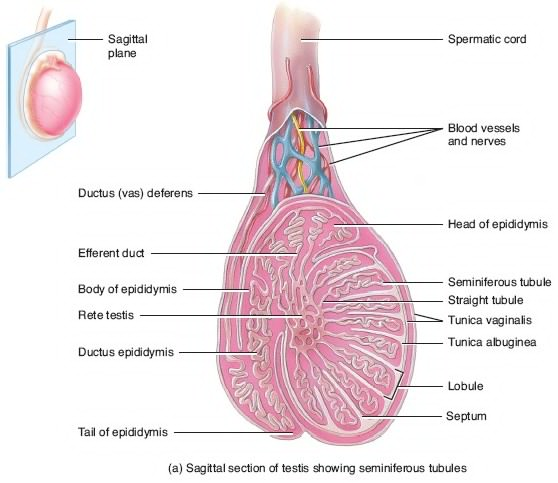
\includegraphics[scale=0.65]{figure/coupe_testicule2} 
  
  }
  
  \caption{Schéma anatomique du testicule humain : }\label{fig:testicule}
  \end{figure}
  
  \subsection{La phase de
  multiplication}\label{la-phase-de-multiplication}
  
  La phase de multiplication est la phase au cours de laquelle les
  spermatogonies se divisent par mitoses pour aboutir au stade de
  spermatocytes primaires. Les spermatogonies sont des cellules diploïdes
  à l'origine de l'ensemble des autres cellules germinales humaines. Pour
  cela, elles vont s'auto-renouveler par mitose successive afin de
  maintenir une production continue de spermatozoïdes tout au long de la
  vie de l'individu. Ces cellules sont localisées dans le compartiment
  basal des tubes séminifères. Les analyses histologiques ont permis de
  distinguer trois types de spermatogonies en fonction de leur contenu en
  hétérochromatine ((Clermont, 1963, Clermont (1966), Goossens \& Tournaye
  (2013))) :
  
  \begin{enumerate}
  \def\labelenumi{\arabic{enumi}.}
  \tightlist
  \item
    Les spermatogonies de type A dark (ou Ad)\\
  \item
    Les spermatogonies de type A pale (ou Ap)\\
  \item
    Les spermatogonies de type B
  \end{enumerate}
  
  Chez l'Homme, les spermatogonies Ad ont une activité mitotique au cours
  de la spermatogénèse et servent de réserve. Elles vont au cours d'une
  première mitose former une spermatogonie Ad et un spermatogonie Ap
  (\textbf{Figure :} \ref{fig:spermatogenese}). Cette propriété permet à
  la fois de se différencier en spermatocytes tout en constituant un
  compartiment de réserve de spermatogonies Ad pour la régénération de la
  population de cellules germinales au sein de l'épithélium séminifère.
  L'entrée en division des spermatogonies Ap se fait par groupes
  cellulaire tous les 16 jours. Les cellules d'une même génération
  maintiennent entre elles des ponts cytoplasmiques jusqu'à la
  spermiogénèse ce qui permet la synchronisation parfaite du développement
  gamétique de toutes les cellules filles issues d'un groupe de
  spermatogonies Ap. Ce phénomène est appelé onde spermatogénétique.
  Chaque spermatogonie Ap va, lorsqu'elle se divise par mitose, former
  deux spermatogonies B qui elles-mêmes se diviseront en deux
  spermatocytes primaires diploïdes (\textbf{Figure :}
  \ref{fig:spermatogenese}).
  
  \begin{figure}
  
  {\centering 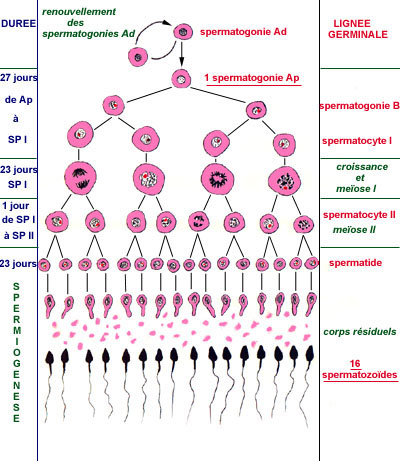
\includegraphics[scale=0.75]{figure/spermatogenese} 
  
  }
  
  \caption{Les différentes phases de la spermatogénèse (À CHANGER !!!!!)}\label{fig:spermatogenese}
  \end{figure}
  
  \subsection{La méïose}\label{la-meiose}
  
  La méiose, ou phase de maturation, est l'étape au cours de laquelle, à
  partir de cellules diploïdes (les spermatogonies B) vont se former des
  cellules haploïdes, les spermatocytes secondaire (spermatocytes II). Ce
  résultat est le fruit de deux divisions successives (\textbf{Figure :
  }@ref(fig:méiose)) appelée respectivement méiose réductionnelle ou
  méiose I (MI) et méiose équationnelle ou méiose II (MII). La MI va
  séparer les chromosomes homologues, produisant deux cellules et
  réduisant la ploïdie de diploïde à haploïde (d'où son non
  \emph{réductionelle}). En plus de son rôle de division vu précédemment,
  la méiose joue un rôle clef dans le brassage génétique (mélange des
  gènes) et ce, grâce à deux mécanismes de brassage : le brassage
  inter-chromosomique, lorsque les chromosomes sont séparés et le brassage
  intra-chromosomique impliquant notamment des enjambements chromosomiques
  (crossing-over) (\textbf{Figure : }\ref{fig:crossingover}).
  
  \begin{figure}
  
  {\centering 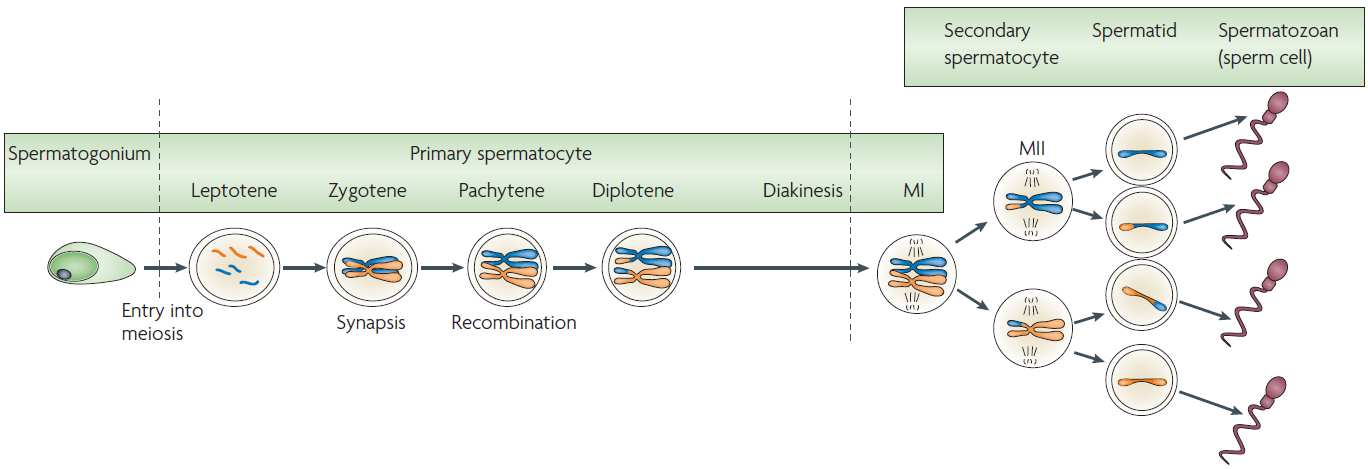
\includegraphics[scale=0.35]{figure/Meiosis_Stages} 
  
  }
  
  \caption[Les différentes étapes de la méiose gamétique masculine]{Les différentes étapes de la méiose gamétique masculine : D’après Sasaki et Matsui,2008}\label{fig:meiose}
  \end{figure}
  
  La méiose est initié dès la fin de la phase de multiplication à partir
  des spermatocytes primaires issus de la division des spermatogonies de
  type B. Ces cellules nouvellement formées se situent dans le
  compartiment basal du tube séminifère. C'est là qu'ils vont tout d'abord
  subir une interphase (stade préleptotène) durant entre 2 à 4 jours. Au
  cours de cette phase a lieu la réplication de l'ADN. Cette réplication
  se fait lorsque l'ADN est à l'état de chromatine, pendant la phase S
  (pour synthèse) de l'interphase. À l'issue de cette phase, chaque
  chromosome sera composé de deux chromatides reliées entres elles par le
  centromère, le matériel génétique de chaque cellules ayant donc été
  multiplié par 2. Par la suite, ces cellules vont subir deux divisions
  méiotiques, chacune composées de 4 étapes distincte (\textbf{Figure :
  }\ref{fig:mitose}) :
  
  \begin{enumerate}
  \def\labelenumi{\arabic{enumi}.}
  \tightlist
  \item
    La prophase, caractérisée par la condensation de la chromatine formant
    ainsi les chromosomes.\\
  \item
    La métaphase, phase au cours de laquelle les chromosomes vont
    s'aligner à l'équateur de la cellule pour former la plaque
    équatoriale.
  \item
    L'anaphase, les chromatides sœurs (ou les chromosomes homologues en
    fonction de la phase méiotique) vont se séparer et migrer aux pôles
    opposés de la cellule.\\
  \item
    La télophase, qui est l'étape finale, les chromosomes se décondensent
    et l'enveloppe nucléaire se reforme autours des chromosomes. La
    cellule mère se sépare alors en deux cellules filles.
  \end{enumerate}
  
  \begin{figure}
  
  {\centering 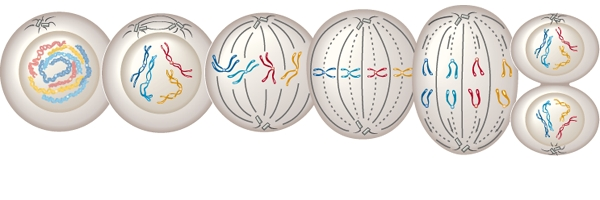
\includegraphics[scale=.55]{figure/phases_mitose} 
  
  }
  
  \caption[Les différentes phases de la division cellulaire]{Les différentes phases de la division cellulaire : De la prophase (à gauche) à la télophase (à droite)}\label{fig:mitose}
  \end{figure}
  
  La première division méiotique aboutit à la formation des spermatocytes
  secondaires (spermatocytes II). À ce stade, les cellules sont haploïdes
  et chaque chromosome est composé de deux chromatides sœurs. Après, cette
  brève étape (environ 1 jour) ainsi qu'une très courte interphase sans
  réplication de l'ADN, les spermatocytes II vont entrer en deuxième
  division méiotique. Cette deuxième division est très semblable à une
  division mitotique. La prophase II, à la différence de la prophase I,
  est très courte. Lors de cette étape, les chromosomes constitués de
  chromatides sœurs se dirigent vers la plaque équatoriale. En métaphase
  II, les chromosomes s'alignent au niveau de leurs centromères. En
  anaphase II, les chromatides sœurs se séparent l'une de l'autre et
  migrent vers les pôles opposés des spermatocytes II. Lors de la
  télophase II, on observe la formation de cellules filles haploïdes
  appelées spermatides, contenant chacune n chromosomes.
  
  \begin{figure}
  
  {\centering 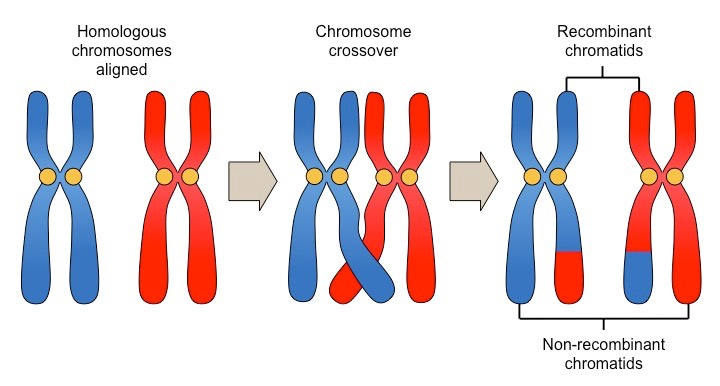
\includegraphics[scale=0.35]{figure/crossingover} 
  
  }
  
  \caption{Schéma simplifé d'un enjambement chromosomique}\label{fig:crossingover}
  \end{figure}
  
  \subsection{La spermiogénèse}\label{la-spermiogenese}
  
  La spermiogénèse est la phase finale de la spermatogénèse. Elle dure
  environs 23 jours chez l'humain et peut être subdivisée en sept étapes
  (\textbf{Figure : }\ref{fig:spermiogenese}). La spermiogénèse définie la
  cytodiférentiation des spermatides en spermatozoïdes. C'est au cours de
  cette phase que les caractéristiques morphologique et fonctionnelles du
  spermatozoïde seront déterminées (Clermont \& Oko 1993 à trouver !!!).
  Elle est caractérisée par 3 évènements majeurs : la formation de
  l'acrosome, la compaction de l'ADN nucléaire et la formation du
  flagelle. Le développement de l'acrosome et la formation du flagelle
  commence au niveau des spermatides rondes(Escalier et al., 1991).
  pendant l'élongation de la spermatide, le noyau se condense et devient
  hautement polarisé (Hamilton, D. W., Waites, 1990).\\
  Les spermatides sont situées dans le compartiment adluminal, à proximité
  de la lumière du tube séminifère. Ce sont de petites cellules (8 à 10
  \(\upmu\)m) que l'on peut schématiquement diviser en trois classes :
  
  \begin{enumerate}
  \def\labelenumi{\arabic{enumi}.}
  \tightlist
  \item
    les spermatides rondes (\textbf{Figure : }\ref{fig:spermiogenese} 1-2)
    : L'identification de ces ces cellules représente un difficulté
    technique. Elles ont cependant pu être décrites en détaille par
    différentes techniques de coloration sous microscope optique
    ((Clermont, 1963), (Papic, Katona, \& Skrabalo, 1988), (Schenck \&
    Schill, n.d.), (Adelman \& Cahill, 1989), (World Health Organization,
    1992)). Plusieurs études animales on pu démontrées le potentiel des
    spermatides rondes à donner la vie à des individus sains et fertiles,
    ((a Ogura, Matsuda, \& Yanagimachi, 1994), (A. Ogura, Matsuda, Asano,
    Suzuki, \& Yanagimachi, 1996), (Sasagawa \& Yanagimachi, 1997)), la
    même chose ayant été également observée plus récemment chez l'homme
    ((A. Tanaka et al., 2015)) bien que le taux de fécondation et
    d'implantation soit extrêmement faible((Asimakopoulos, 2003)). Ils
    possèdent un noyau rond avec une chromatine pâle et homogène. C'est à
    partir de ces étapes que démarre la biogenèse de l'acrosome avec la
    production par l'appareil de Golgi des vésicules pro-acrosomales
    (phase de Golgi). Les deux centrioles contenus dans le cytoplasme vont
    se déplacer au futur pôle caudal. Le centriole proximal est inactif
    alors que le centriole distal donne naissance à un ensemble de
    microtubules à l'origine de l'axonème du futur flagelle.\\
  \item
    Les spermatides en élongation (\textbf{Figure :
    }\ref{fig:spermiogenese} 3-4) :\\
    peuvent aussi donner naissance avec un meilleur taux que les
    spermatides rondes et engendrerai théoriquement moins de risques
    d'anomalies génétiques ((Asimakopoulos, 2003)). \textbf{A completer}\\
  \item
    Les spermatides en condensation (\textbf{Figure :
    }\ref{fig:spermiogenese} 5-7) : C'est le stade final de la
    différentiation du spermatide en spermatozoïde. À ce stade le noyau
    est très allongé, avec une partie caudale globulaire et une partie
    antérieure saillante. La chromatine est sombre et condensée. L'axonème
    va continuer à s'allonger pour former le flagelle mature. Les
    différentes organelles inutiles pour la physiologique spermatique et
    l'excès de cytoplasme vont former la gouttelette cytoplasmique qui va
    se détacher et donner le corps résiduel qui va ensuite être phagocyté
    par les cellules de Sertoli ((Hermo, Pelletier, Cyr, \& Smith, 2010)).
  \end{enumerate}
  
  Une fois ces étapes de différentiation finies, les spermatides sont
  relachées en tant que spermatozoïdes dans la lumière du tube séminifère.
  Ce procédé est appelé spermiation.
  
  \begin{figure}
  
  {\centering 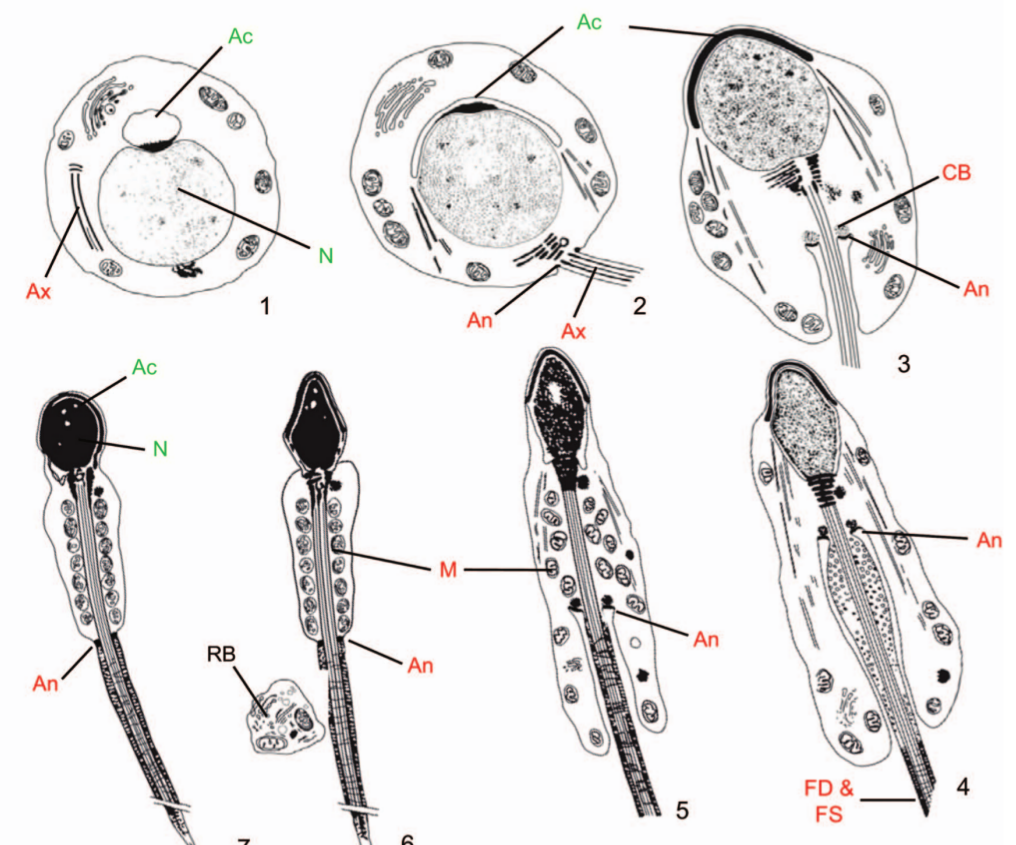
\includegraphics[scale=0.3]{figure/spermiogenese} 
  
  }
  
  \caption[Principales étapes et modifications structurales lors de la spermiogénèse]{Principales étapes et modifications structurales lors de la spermiogénèse : 1. La spermatide immature avec un gros noyau arrondi. La vésicule acrosomale est attachée au noyau, l’ébauche du flagelle n’atteint pas le noyau. 2. La vésicule acrosomale a augmenté de taille et apparaît aplatie au niveau du noyau. Le flagelle entre en contact avec le noyau. 3-7. Formation de l’acrosome, condensation du noyau et développement des structures flagellaires. Ac, acrosome; Ax, axonème; CC, corps chromatoïdes; CR, corps résiduel; FD, fibres denses; GF, gaine fibreuse; M, mitochondrie; Ma, manchette. D’après Touré et al., 2011}\label{fig:spermiogenese}
  \end{figure}
  
  \section{Structure et fonction du
  spermatozoïde}\label{structure-et-fonction-du-spermatozoide}
  
  \subsection{Anatomie du spermatozoïde}\label{anatomie-du-spermatozoide}
  
  Une fois Il est composé de deux parties principales : La tête et le
  flagelle (\textbf{Figure : }\ref{fig:spz}).
  
  \begin{figure}
  
  {\centering 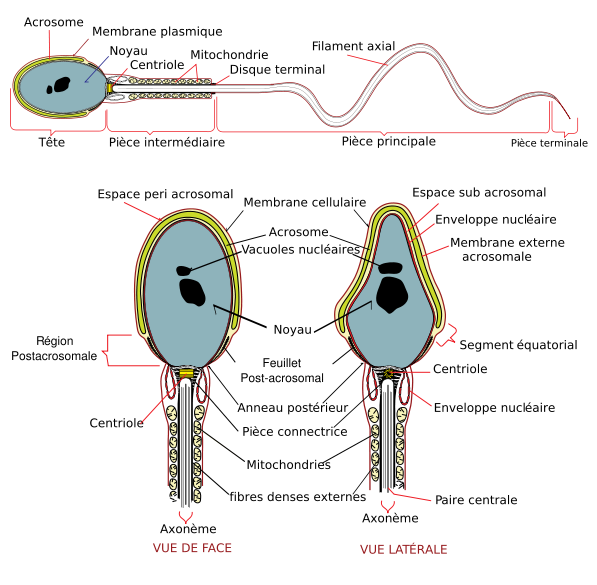
\includegraphics[scale=.6]{figure/spermatozoide} 
  
  }
  
  \caption[Anatomie du spermatozoïde]{Anatomie du spermatozoïde}\label{fig:spz}
  \end{figure}
  
  \subsubsection{La tête}\label{la-tete}
  
  \begin{enumerate}
  \def\labelenumi{\arabic{enumi}.}
  \tightlist
  \item
    L'acrosome : C'est une vésicule de sécrétion géante située dans la
    moitiée superieur de la tête du spermatozoïde. Elle se développe à
    partir de l'appareil de Golgi lors de la spermiogénèse. Au cours de sa
    formation, l'acrosome forme tout d'abord un granule sphérique qui se
    colle sur la partie apical du noyau. En s'aplatissant contre celui-ci,
    l'acrosome va prendre une forme hémishpérique recouvrant la membrane
    nucléaire formant la coiffe céphalique\ldots{} Le rôle de l'acrosome
    est fondamental dans le processus de fécondation puisqu'il permet
    d'excréter nottament l'acrosine, une enzyme de digestion permettant au
    spermatozoïde de pénétrer la zone pellucide qui entoure les ovocytes.
    Ce processus de relargage est appelé réaction acrosomal.\\
  \item
    L'acroplaxome : \textbf{TODO !!!}\\
  \item
    Le noyau : Le noyau est une structure cellulaire présente dans la
    majorité des cellules eucaryotes. Il contient l'essentiel du materiel
    génétique. Le noyau du spermatozoïde est caractérisé par une
    compaction extrêmement importante de l'ADN. Dans les cellules
    somatiques l'ADN est enroulé par unité de 146 paires de bases autour
    d'un octamère d'histones dit de cœur (H2A, H2B, H3 et H4) afin
    d'organiser les 3 milliards de paires de bases du génome humain dans
    un noyau de quelques microns (\textbf{Figure : }\ref{fig:noyau}).
    L'ADN des spermatides va subir une réorganisation chromatinienne plus
    importante au cours de la spermatogénèse afin d'augmenter sa
    compaction. Ainsi, les octamères d'histones présents dans les cellules
    somatiques sont remplacées par deux protéines riches en arginine et en
    cystéine PRM1 et PRMM2). Ces protéines sont appellées des protamines
    (\textbf{Figure : }\ref{fig:noyau}). L'intégrité des deux protéines
    composant ce dimère est nécéssaire pour la procréation (Cho et al.,
    2001). Cette compaction extrême permet de réduire la taille du noyau,
    mais aussi de protéger l'ADN d'agents de dégradation comme l'oxydation
    des bases. Parallèlement à cette condensation chromatinienne se
    produit un arrêt des processus de transcription cellulaire
    ((Kierszenbaum \& Tres, 1978)). Le noyau du spermatozoïde est donc un
    noyau au repos, transcriptionnellement inactif ((Ward, 1994))
  \end{enumerate}
  
  \begin{figure}
  
  {\centering 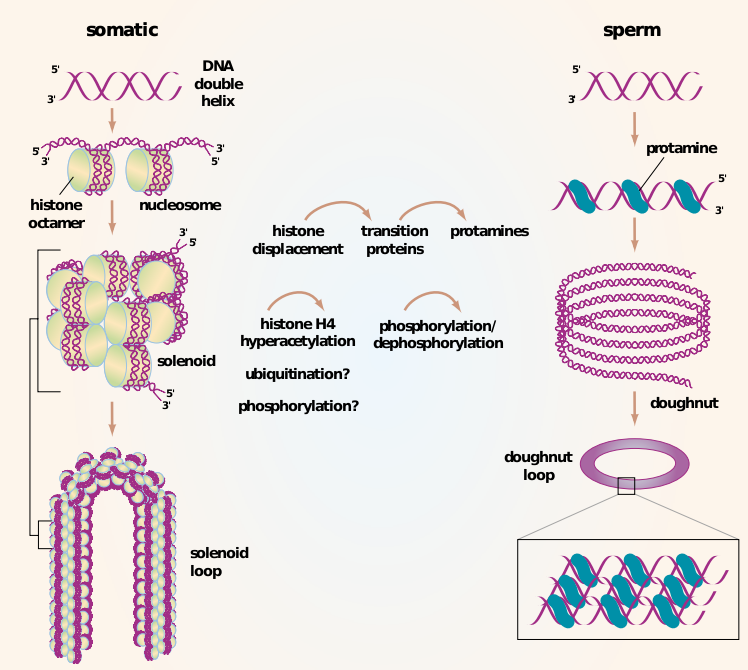
\includegraphics[scale=.55]{figure/noyau} 
  
  }
  
  \caption[Schéma de la compaction de l’ADN dans les cellules somatiques et dans les
  spermatozoïde]{Schéma de la compaction de l’ADN dans les cellules somatiques et dans les
  spermatozoïde : D'après Braun (2001)}\label{fig:noyau}
  \end{figure}
  
  \subsubsection{Le flagelle}\label{le-flagelle}
  
  Le flagelle représente la queue du spermatozoïde. Celui-ci permet, par
  mouvement d'oscilation à haute vitesse, le déplacement du spermatozoïde.
  Cette mobilité est générée par un cytosquelette interne extrêmement
  conservé durant l'évolution appelée l'axonème. Celui-ci est composé de
  neuf doublets de microtubules périphériques et de deux doublets internes
  (Inaba, 2003) (\textbf{Figure : }\ref{fig:axoneme}), on parle alors de
  structure ``9 + 2''. Les doublets externes sont reliés entre eux par des
  ponts de nexine et au doublet central par des ponts radiaires.
  
  \begin{figure}
  
  {\centering 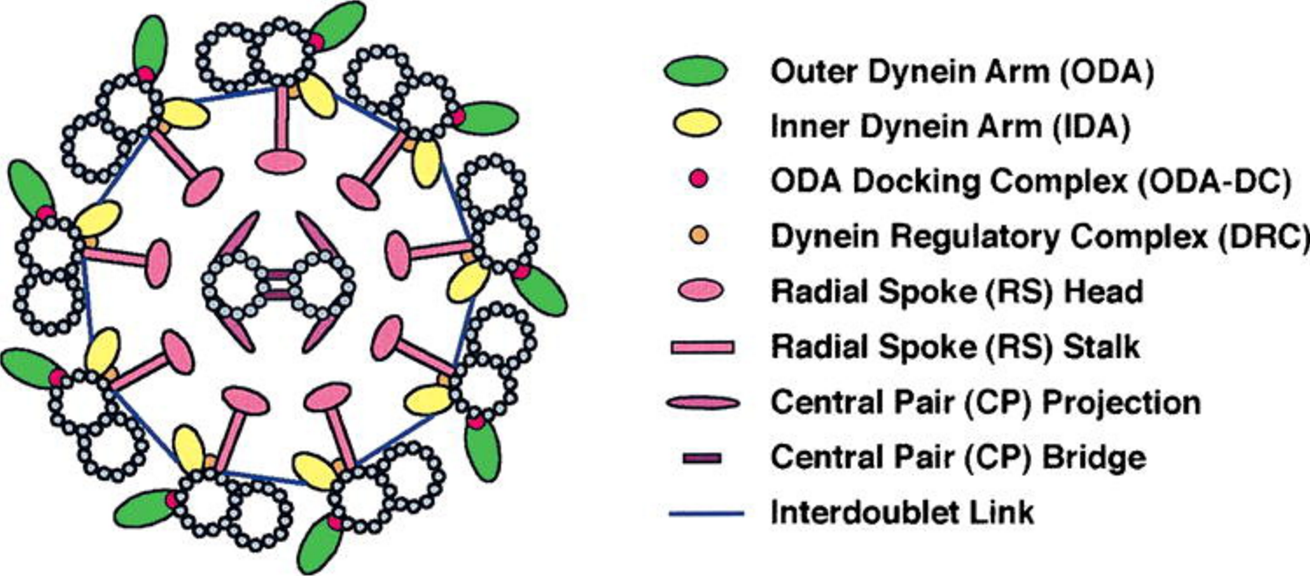
\includegraphics[scale=.3]{figure/axoneme} 
  
  }
  
  \caption[Structure simplifiée de l'axonème d'après Inaba (2003)]{L'axonème es constitué de neuf doublets de microtubules périphériques reliés entre eux par des liens de nexine d'un doublet central relié aux doublets périphériques par des ponts radiaires}\label{fig:axoneme}
  \end{figure}
  
  Le flagelle su spermatozoïde peut être divisé en trois partie distinctes
  (\textbf{Figure : }\ref{fig:flagelle}) :
  
  \begin{enumerate}
  \def\labelenumi{\arabic{enumi}.}
  \tightlist
  \item
    La pièce intermédiaire : Elle fait jonction avec la tête du
    spermatozoïde et est composée de la gaine de mitochondrie qui fournira
    une partie de de l'énergie nécéssaire au batement flagellairee (grâce
    à la phosphorylation oxydative qui produit de l'ATP), l'axonème qui se
    prolonge dans la pièce principale et un ensemble de neuf faisceaux de
    fibres denses.\\
  \item
    La pièce principale : Ici, la gaine de mitochodrie a disparue ainsi
    que deux des faisceaux de fibres denses présents dans la pièce
    intermédiaire. On note cependant la présence d'une structure
    suplémentaire, la gaine fibreuse. Cette gaine entoure l'axonème et
    comporte deux épaississements diamétralement opposés, appelées
    colonnes longitudinales sur lesquelles s'insère les fibres denses 3 et
    8. C'est le long de la gaine fibreuse qu'est produit la majorité de
    l'énergie 46nécessaire au glissement des microtubules ((Eddy,
    2007)).\\
  \item
    La pièce terminale : Elle est située au niveau'de l'extrémité distale
    du flagelle et ne contient que l'axonème (Inaba, 2003).
  \end{enumerate}
  
  \begin{figure}
  
  {\centering 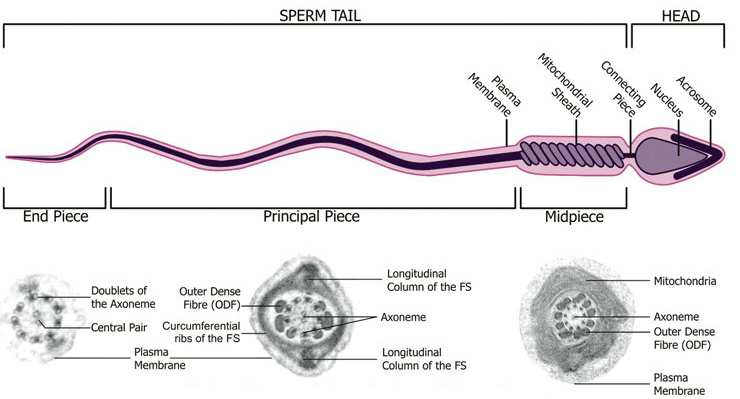
\includegraphics[scale=.55]{figure/sperm2} 
  
  }
  
  \caption[Structure du flagelle d’un spermatozoïde d’après Borg et al. (2010)]{Structure du flagelle d’un spermatozoïde d’après Borg et al. (2010) : Coupes transversales en microscopie électronique. Le flagelle se compose de trois parties : la pièce intermédiaire, contenant les mitochondries, la pièce principale et la pièce terminale. L’axonème, en position centrale, parcours tout le flagelle. Des structures périaxonèmales sont observables : les fibres denses dans la pièce intermédiaire et principale, et la gaine fibreuse dans la pièce principale seulement.}\label{fig:flagelle}
  \end{figure}
  
  \subsection{Fonction du spermatozoïde}\label{fonction-du-spermatozoide}
  
  En plus d'être unique dans sa morphologie, le spermatozoïde l'est aussi
  dans sa fonction puisque c'est la seule cellule produite de manière
  endogène et dont l'action est exercée de manière exogène.
  
  \section{L'infertilité masculine}\label{linfertilite-masculine}
  
  L'organisation mondiale de la santé définie l'infertilité comme étant :
  ``\emph{une pathologie du système reproductif définie par l'échec d'une
  grossesse clinique après 12 mois ou plus de rapports sexuels réguliers
  non protégés}''
  (\href{http://www.who.int/reproductivehealth/topics/infertility/definitions/en/}{\texttt{Who.int.\ 2013-03-19.\ Retrieved\ 2013-06-17}}).
  Environ 10-15\% des couples humains sont considérés infertiles. On
  estime que dans la moitié des cas, la cause sous-jacente est masculine.
  Les facteurs causaux sous-jacents de l'infertilité masculine peuvent
  être attribués à des toxines environnementales, des troubles systémiques
  tels que la maladie hypothalamo-hypophysaire, les cancers testiculaires
  et l'aplasie des cellules germinales. Les facteurs génétiques, y compris
  les aneuploïdies et les mutations de gènes uniques, contribuent
  également à l'infertilité masculine. Cependant, aucune cause n'est
  identifiée dans 10-20\% des cas.
  
  The entire process (of spermatogenesis) is tightly synchronized and
  integrated, so that pathological conditions which produce even very
  small deviations are likely to lead to infertility (Barratt, 1995)\\
  Barratt, C.L.R. (1995) Spermatogenesis. In Grudzinsky, J.G. and Yovich,
  J.L. (eds) Gametes: the spermatozoon. Cambridge University Press,
  Cambridge
  
  \subsection{Les différents phénotypes d'infertilité
  masculine}\label{les-differents-phenotypes-dinfertilite-masculine}
  
  \subsubsection{Liée à la quantité}\label{liee-a-la-quantite}
  
  Immature germ cells are present in ejaculates of subjects with a normal
  sperm count (Michael and Joel, 1937; Tomlinson et al., 1992),
  oligozoospermia (Mac Leod, 1970; Tomlinson et al., 1993), or azoospermia
  (Kurilo et al., 1993) and the presence of immature germ cells increases
  as the sperm count decreases (Sperling and Kaden, 1971) Michael, M. and
  Joel, K. (1937) Zellformen in normalen und pathologischen Ejakulaten und
  ihre klinische Bedeutung. Schweiz. Med. Wsch., 33, 757.\\
  Tomlinson, M.J., Barratt, C.L.R., Bolton, A.E. et al. (1992) Round cells
  and sperm fertilizing capacity: the presence of immature germ cells but
  not seminal leukocytes are associated with reduced success of in vitro
  fertilization. Fertil. Steril., 58, 1257--1259.\\
  MacLeod, J. (1970) The significance of deviations in human sperm
  morphology. In: Rosemberg, E. and Paulsen, C.A. (eds) The human testis.
  Plenum, New York, pp.~481--494.\\
  Tomlinson, M.J., Barratt, C.L.R. and Cook, I.D. (1993) Prospective study
  of leukocytes and leukocyte populations in semen suggests they are not a
  cause of male infertility. Fertil. Steril., 60, 1069--1075\\
  Kurilo, L.F., Liubashevskaia, I.A., Dubinskaia, V.P. and Gaeva, T.N.
  (1993) Karyological analysis of the count of immature germ cells in the
  ejaculate. Urol. Nefrol. (Mosk.), 2, 45--47.\\
  Sperling, K. and Kaden, R. (1971) Meiotic studies of the ejaculated
  seminal fluids of humans with normal sperm count and oligospermia.
  Nature, 232, 481
  
  In humans, spermatogenic arrest was considered a hopeless condition for
  couples desiring to conceive. However, the documented success of
  intracytoplasmic sperm injection (ICSI; Palermo et al., 1992) has
  pointed to using this technique to inject spermatids into oocytes
  (Edwards et al. 1994; Ogura et al., 1994) Palermo, G., Joris, H.,
  Devroey, P. and Van Steirteghem, A.C. (1992) Pregnancies after
  intracytoplasmic sperm injection of a single spermatozoon into an
  oocyte. Lancet, 340, 17--18.\\
  Edwards, R.G., Tarin, J.J., Dean, N. et al. (1994) Are spermatids
  injections into human oocytes now mandatory? Hum. Reprod., 9,
  2217--2219.\\
  Ogura, A., Matsuda, J. and Yanagimachi, R. (1994) Birth of normal young
  after electrofusion of mouse oocytes with round spermatids. Proc. Natl.
  Acad. Sci. USA, 91, 7460--7462
  
  Spermatogenic arrest, the inability of spermatogenetic cells to develop
  into male gametes within the gonads, has been reported in 4--30\% of
  testicular biopsies of patients with severe oligospermia or azoospermia
  (Wong et al., 1973; Levin, 1979; Colgan et al., 1980; Soderstrom and
  Suominen, 1980; Nomen et al., 1984) Wong, T.W., Strauss, F.H. and Worne,
  N.E. (1973) Testicular biopsy in male infertility: I. Testicular causes
  of infertility. Arch. Pathol. Lab. Med., 95, 151--159.\\
  Levin, H.S. (1979) Testicular biopsy in the study of male infertility.
  Hum. Pathol., 10, 569--579\\
  Colgan, T.J., Bedar, Y.C., Strawbridge, H.T.G. et al. (1980) Reappraisal
  of the value of the testicular biopsy in the investigation of
  infertility. Fertil. Steril., 33, 56--60.\\
  Soderstro¨m, K.O. and Suominen, J. (1980) Histopathology and
  ultrastructure of meiotic arrest in human spermatogenesis. Arch. Pathol.
  Lab. Med., 104, 476--482.\\
  Soderstro¨m, K.O. and Suominen, J. (1980) Histopathology and
  ultrastructure of meiotic arrest in human spermatogenesis. Arch. Pathol.
  Lab. Med., 104, 476--482.
  
  Spermatogenic arrest can occur at any stage of germ cell formation;
  primary spermatocyte arrest is most prominent, followed by spermatid
  arrest, and least commonly, spermatogonial arrest. Arrest at primary
  spermatocyte stage can be incomplete, so that a few secondary
  spermatocytes or spermatids are observed (Girgis et al., 1969)\\
  Girgis, S.M., Etriby, A., Ibrahim, A.A. and Kahil, A. (1969) Testicular
  biopsy in azoospermia. A review of the last ten years' experience of
  over 800 cases. Fertil. Steril., 20, 467--477.
  
  \subsubsection{liée à la forme}\label{liee-a-la-forme}
  
  teratozoospermia
  
  \paragraph{La globozoospermie}\label{la-globozoospermie}
  
  La globozoospermie est une anomalies des spermatozoïdes caractérisé par
  une tête ronde dépourvue d'acrosome et d'une pièce intermédiaire
  désorganisiée ((Singh, n.d.), (Pedersen \& Rebbe, 1974))
  
  \subsubsection{liée à la mobilitée}\label{liee-a-la-mobilitee}
  
  Sperm motility is necessary for the transport of male DNA to eggs in
  species with both external and internal fertilization.
  
  \subsection{La génétique de
  l'infertilité}\label{la-genetique-de-linfertilite}
  
  \subsubsection{Les causes fréquentes}\label{les-causes-frequentes}
  
  \paragraph{Les microdélétions du chromosome
  Y}\label{les-microdeletions-du-chromosome-y}
  
  \paragraph{Anomalies chromosomiques}\label{anomalies-chromosomiques}
  
  \paragraph{Mutations CFTR}\label{mutations-cftr}
  
  \subsubsection{Les nouveaux gènes}\label{les-nouveaux-genes}
  
  \begin{center}\rule{0.5\linewidth}{\linethickness}\end{center}
  
  \section{Les techniques d'analyses
  génétiques}\label{les-techniques-danalyses-genetiques}
  
  L'acide desoxyribonucléique (ADN) a été identifié comme étant le porteur
  de l'information génétique par Oswald Theodore Avery en 1944. Sa
  structure en double hélice composée par quatre bases, la thymine,
  l'adénine, la guanine et la cytosine fut caractérisée en 1953 par James
  D. Watson et Francis Crick
  
  \subsection{Les puces}\label{les-puces}
  
  \begin{enumerate}
  \def\labelenumi{\arabic{enumi}.}
  \tightlist
  \item
    Bref historique de la technologie\\
  \item
    A quoi ça sert
  \item
    Comment ça marche
  \end{enumerate}
  
  \subsubsection{Les puces à SNP, le génotypage\ldots{} (titre à
  revoir)}\label{les-puces-a-snp-le-genotypage-titre-a-revoir}
  
  \subsubsection{Du tissu au transcriptome, le différentiel
  d'expression}\label{du-tissu-au-transcriptome-le-differentiel-dexpression}
  
  \subsection{Le séquençage NGS}\label{le-sequencage-ngs}
  
  Le terme séquençage de l'ADN fait référence à l'enssemble des technique
  permettant de déterminer l'ordre des nucléotides adenine (A), tymine
  (T), cytosine (C) et guanine (G) de l'integralité ou d'une partie d'une
  molécule d'ADN. Avant de parler des nouvelles technologies de séquençage
  (NGS) faisons un bref historique du séquençage de l'ADN. En 1977
  Frederick Sanger développe une technologie de séquençage d'ADN basée sur
  la méthode \emph{chain-termination}. Ce procédé est desormais connu sous
  le nom de séquençage Sanger. D'autre méthode furent développées à la
  même periode, notamment celle de Walter Gilbert basée sur la
  modification chimique de l'ADN, cependant sa grande efficience et sa
  faible utilisation de la radioactivité permirent au séquençage Sanger de
  s'imposer comme référence dans la ``première génération'' de séquençeur
  à application de commerciale et de recherche
  (\href{http://en.wikipedia.org/wiki/DNA_sequencing}{Wikipedia}). Apparu
  en 1998, les instruments de séquençage automatique ainsi que les
  logiciels associés utilisant le séquençage par capilarité et la
  technologie Sanger furent les outils principaux qui permirent la
  completion du \emph{human genome project} en 2001 (Collins, Morgan, \&
  Patrinos, 2003).
  
  Contrairement à la méthode Sanger, le NGS \emph{lit} des fragment d'ADN,
  provenant d'un génome entier, de manière aléatoire. On parle alors de
  séquençage de génomes entiers ou \emph{whole genome sequencing} (WGS).
  Pour cela, la molécule d'ADN est ``coupée'' en plusieurs fragments d'une
  taille donnée. Ce sont ensuite ces fragments qui seront, après une étape
  d'amplification spécifique au différentes plateformes, séquencés
  simultanément. C'est pourquoi on parle souvent de séquençage parrallèle
  massif pour décrire le NGS. Le produit de ce séquençage est appelé
  \emph{read}. Cette technologie est avantageuse de part la masse de
  \emph{reads} qu'elle produit et par son faible cout par bases séquencées
  (Metzker, 2010). Ces caractéristiques ont permis au séquençage
  Haut-débit d'être courmment utilisé dans le domaine de la recherche
  clinique. La taille des \emph{reads} obtenus par séquençage NGS est
  nettement inferieure à celle atteinte par le séquençage Sanger. À
  l'heure actuelle, les \emph{reads} aobtenus par séquençage NGS ont une
  taille comprise entre 50 et 500 pb pour la plupart des plateforme contre
  \ldots{} obtenus par Sanger (\textbf{Figure :} \ref{fig:readPerRun}),
  c'est pour cela que les résultats du séquençage NGS sont appelés des
  \emph{reads} courts ou \emph{short reads}.\\
  Étant donnée que le NGS produit à l'heure actuelle des \emph{reads}
  courts la notion de couverture est importante et représente l'un des
  critère majeur à considérer dans l'analyse des données (Sims, Sudbery,
  Ilott, Heger, \& Ponting, 2014). La couverture est définie comme le
  nombre de \emph{reads} qui, après l'atape d'alignement
  \protect\hyperlink{lalignement}{cf alignment}, se chevauchent les uns
  les autres au sein du région génomique spécifique. Par exemple, une
  couverture de 30x pour le gène \emph{XXXX} signifie que chaque
  nucléotide de ce gène est chevauchés par au moins 30 \emph{reads}
  distincts.
  
  \begin{figure}
  
  {\centering 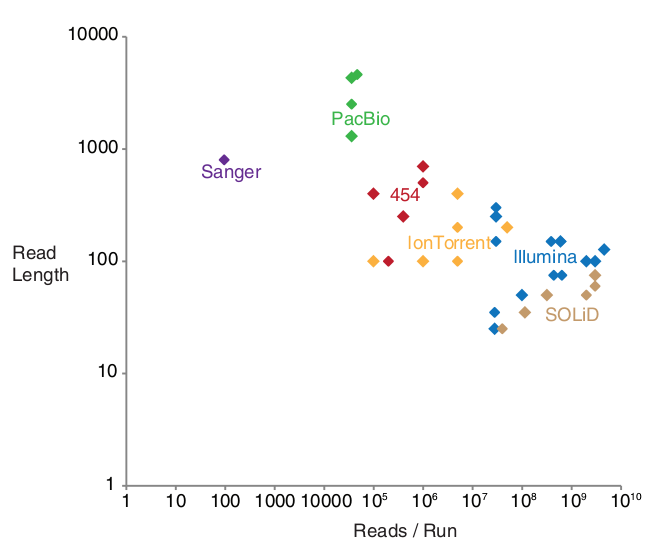
\includegraphics[scale=.55]{figure/read_per_run} 
  
  }
  
  \caption[Présentation de la taille des reads et du nombre de reads par run en fonction de la technologie de séquençage utilisée]{Présentation de la taille des reads et du nombre de reads par run en fonction de la technologie de séquençage utilisée d'après Brendan et. al, (2014) : Sequencing space based on read length (in bases) and number of reads per run. Points represent official platform/chemistry combination releases and are color-coded based on the platform family. To see this illustration in color, the reader is referred to the web version of this article at www.liebertpub.com/wound}\label{fig:readPerRun}
  \end{figure}
  
  \subsubsection{La capture des parties à séquencer, avantage et
  inconvegnants}\label{la-capture-des-parties-a-sequencer-avantage-et-inconvegnants}
  
  Pour de nombreuses application, il peut être intérésesant de ne
  séquencer qu'une partie du génome et non pas son intégralité. Dans cette
  sous partie de génome ciblé on peut trouver par exemple : une région
  génomique spécifique à laquelle une pathologie a déjà été associé,
  l'ensembles des exons de certains gènes candidats, ou encore
  l'intégralité des exons de l'ensemble des gènes codant pour une
  protéine.Dans ce dernier cas on parle alors de séquençage exomique ou
  \emph{whole exome sequencing} (WES). Les principaux avantages du WES par
  rapport au WGS sont son cout réduits ainsi qu'une masse de données moins
  importantes à stocker et à analyser. En effet, l'ensemble de l'exome ne
  représente qu'environs 1\% du génome entier. Pour ces raisons, le WES
  considéré comme le standard dans le cadre de recherche sur des
  pathologies génétiques et se révèle être un outil puissant pour
  l'identification de variants associés à des pathologies (Ng et al.,
  2010). Le procédé de séquençage est identique au WGS, il est simplement
  précédé d'une étape d'enrichissement au cours de laquelle les exons sont
  capturés par hybridation à des sondes. De fait les exons capturés sont
  donc dépendant du kit de capture utilisé, cette technique permet donc de
  séquencer uniquement les exons connus et ciblés par les sondes. Il faut
  également noté que depuis quelque années, plusieurs étude ont remis en
  cause lk'interet du WES au profis du WGS, nottament car le WGS fournit
  une meilleur couverture sur l'exome que le WES (Lelieveld, Spielmann,
  Mundlos, Veltman, \& Gilissen, 2015, Meienberg, Bruggmann, Oexle, \&
  Matyas (2016)), de plus le WES montre une plus grande sensibilité au
  pourcentage de GC contenu dans la région à séquencer et à la séléction
  des kit de capture utilisés (Meienberg et al., 2016). Ainsi, bien que le
  WES soit encore à l'heure actuelle le choix privilégié dans la majorité
  des études (citation\ldots{}), la réduction des couts de séquençage et
  de stockage des données, il est possible que le WGS remplace totalement
  le WES ainsi que l'ensemble des techniques impliquant la capture de
  séquences ciblées (Meienberg et al., 2016).
  
  \subsubsection{L'amplification}\label{lamplification}
  
  Dans la plupart des technologies, la phase de séquençage est précédée
  par une étape d'amplification de l'ADN. Cette amplification se fait dans
  la grande majoritée des cas sur une surface solide exepté pour la PCR en
  émultion qui s'effectue en phase aqueuse. Elle permet d'obtenir dans une
  région définie plusieurs milliers de copie du même fragment d'ADN,
  appelés des clones. Cette étape assure que le signal emis lors du
  séquençage pourra être distingué du bruit. Chacun de ces \emph{spots}
  d'amplification appelés aussi centre de réaction, se retrouve donc être
  le représentant d'un unique fragment d'ADN et sera ensuite séquencé
  parrallèlement aux autres \emph{spots}. Une platforme de séquençage
  pouvant gérer plusieurs millions de ces centres de réactions
  simultanément, séquençant ainsi plusieurs millions de mollécules d'ADN
  en parrallèle, donnant ainsi le nom à ces techniques qualifiées de
  séquençage massif en parrallèle. Cette étape d'amplification est
  généralement précédée d'une phase de fragmentation de l'ADN. cette
  fragmentation peut-être phisique, enzymatique ou bien chimique. Ce sont
  les résidus d'ADN résultant de cette fragmentation qui seront ensuite
  amplifié. Il existe quatre stratégies utilisées pour le clonage de l'ADN
  dans le cadre du NGS :\\
  1. La PCR en emulsion ou emPCR (\textbf{Figure : }\ref{fig:ngsampli} -
  \textbf{a}) : Le patron d'ADN fragmenté simple brin est lié à une
  séquence adaptatrice complémentaire et est capturé par une goutelette
  aqueuse appelée micelle contenant une bille recouverte d'adaptateur
  complémentaire à celui fixé sur le fragment d'ADN ainsi que tout les
  composant nécéssaire à la réaction de PCR. En respectant un ratio nombre
  de molécule d'ADN / nombre de billes, on va fixer un seul fragment d'ADN
  sur chaque bille. Chacune de ces billes seront donc, en fin de réaction,
  recouverte par plusieurs milliers de copies de la même séquence d'ADN.\\
  2. L'amplification par pont sur face solide (\textbf{Figure :
  }\ref{fig:ngsampli} - \textbf{b}) : Les fragments d'ADN sont liés à des
  séquences adaptatrices et liée par une de leurs extrémités à une amorce
  fixée sur un support solide. Du fait de la dilution, les molécules d'ADN
  se trouvent éloignées les unes des autres. L'extrémitée libre du
  fragment interagit avec les amorces situées à proximité formant une
  structure en pont, d'où le nom de PCR en pont ou \emph{bridge-PCR}. La
  PCR va alors synthétizer un deuxième brin complémentaire aux fragments
  immobilisés sur le support. En procédant à des cycles de température
  comme pour une réaction PCR classique, on obtient à l'emplacement de
  chaque molécule initiale un massif de molécules fixées sur la plaque,
  toutes identiques à la molécule initiale.\\
  3. Amplification par modèle mobile ou \emph{walking-template}
  (\textbf{Figure : }\ref{fig:ngsampli} - \textbf{c}) : L'ADN fragmenté
  est lié à un adaptateur et lié à une amorce complémentaire fixée sur un
  suport solide. Le brin complémentaire du fragment sera synthétisé par
  PCR à partir de l'amorce fixée. La molécule double brin nouvellement
  formée sera ensuite partiellement dénaturée permettant à l'extrémitée
  libre de se fixée à une séquence amorce voisine. Des amorces
  \emph{reverse} sont ensuite utilisées por resynthétiser un fragment
  d'ADN libre à partir des fragments fixés sur le support.\\
  4. (\textbf{Figure : }\ref{fig:ngsampli} - \textbf{d}) : \textbf{PAS DU
  TOUT COMPRIS LE MECHANISME !!! }
  
  \begin{figure}
  
  {\centering 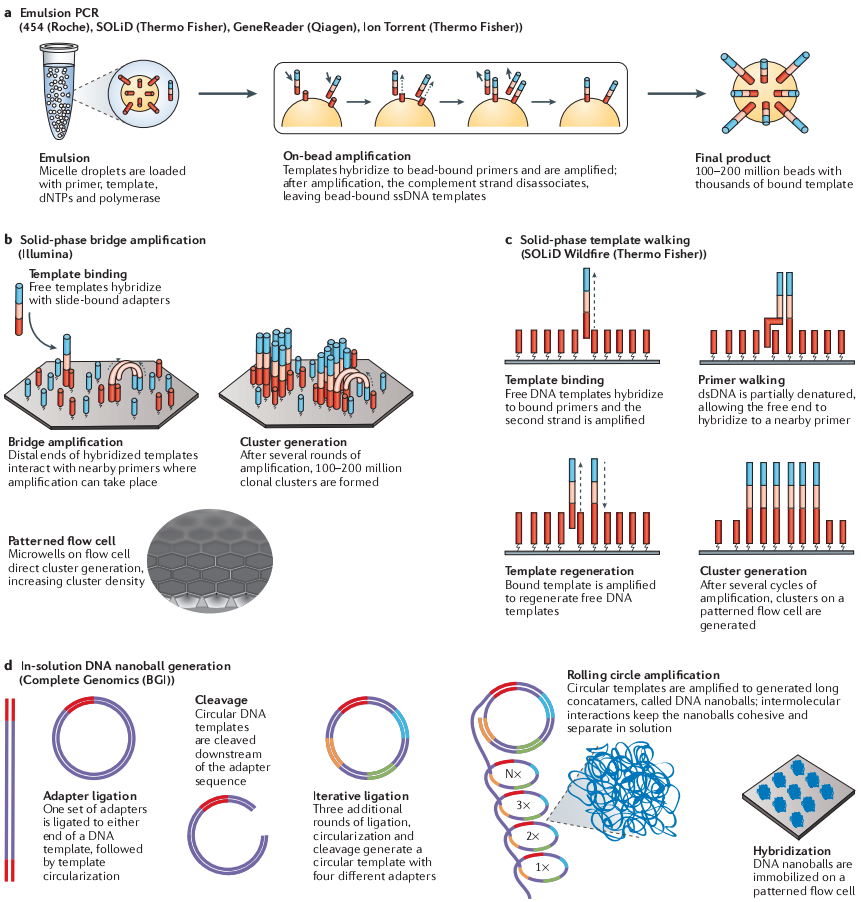
\includegraphics[scale=.545]{figure/ngs_amplification} 
  
  }
  
  \caption[Présentation des différentes stratégies d'amplification de l'ADN dans le cadre du NGS]{Présentation des différentes stratégies d'amplification de l'ADN dans le cadre du NGS d'après [@Goodwin2016] : }\label{fig:ngsampli}
  \end{figure}
  
  \subsubsection{La réaction de séquence}\label{la-reaction-de-sequence}
  
  La réaction de séquence est l'étape suivant l'amplification et consiste
  à déterminer l'ordre dans lequel se succèdent les nucléotides de
  l'ensemble des clones générés dans la phase d'amplification. Il existe
  deux technologies principales permettant le séquençage de \emph{reads}
  courts :\\
  
  \begin{enumerate}
  \def\labelenumi{\arabic{enumi}.}
  \tightlist
  \item
    \textbf{Séquençage par synthèse} (SBS) : Ce type de séquençage
    regroupe l'ensemble des méthodes utilisant l'ADN polymérase pour
    synthetiser de l'ADN. En 2016, Sahra Goodwin et ses collègues ont
    différentiés deux catégories de séquençage par synthèse (Goodwin,
    McPherson, \& McCombie, 2016) :
  
    \begin{enumerate}
    \def\labelenumii{\alph{enumii}.}
    \tightlist
    \item
      \textbf{Terminaison par cycle reversible}, \emph{cyclic reversible
      termination} (CRT) (\textbf{Figure : }\ref{fig:crtSeq}) : Cette
      méthode est caractérisée par son utilisation de molécule dîtes
      terminatrices auxquelles le groupement \(\mathrm{3'-OH}\) est
      modifié de sorte à éviter l'élongation (J. Guo et al., 2008), on
      parlera de groupement \(\mathrm{3'-bloqué}\). Le processus est
      initialisé une amorce est liée au fragment d'ADN et permettra
      l'initialisation de la polymerisation. À chaque cycle, un mixe
      comprenant l'ensemble des quatres de desoxynucléotides (dNTPs),
      préalablement labelisés par uyn fluorophore et
      \(\mathrm{3'-bloqué}\) sont mis en contact du fragment. Après
      l'incorporation d'un unique dNTP au fragment, les dNATP non liés
      sont éliminée et la nature du dNTP ajouté est identifé grace à son
      fluorophore. Le fluorophore et le groupement \(\mathrm{3'-bloqué}\)
      sont retirés permettant ainsi à un nouveau cycle de commencer.
    \end{enumerate}
  \end{enumerate}
  
  \begin{figure}
  
  {\centering 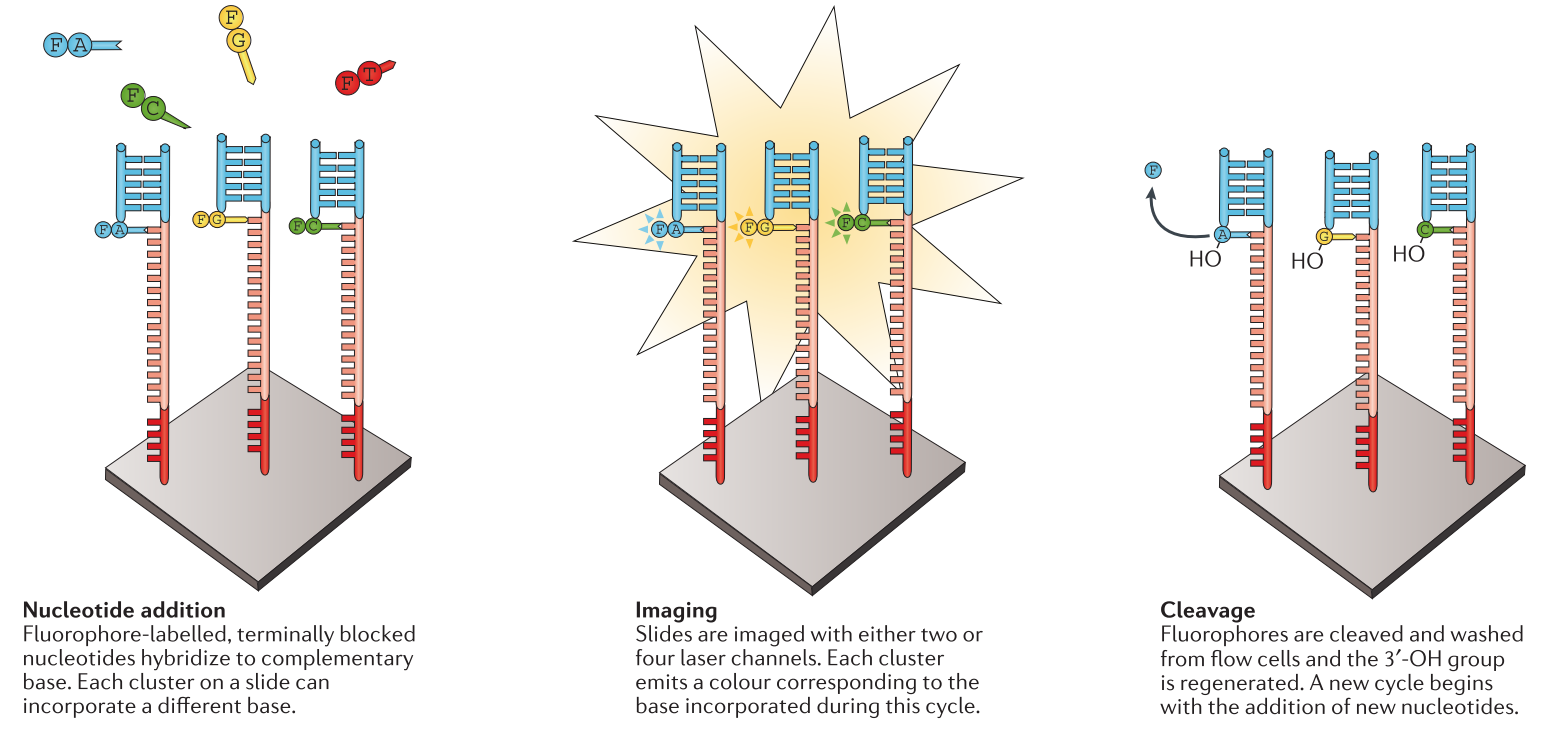
\includegraphics[scale=.28]{figure/CRT_seq_illumina} 
  
  }
  
  \caption[Exemple de séquençage CRT tel qu'il est effectué par Illumina]{Exemple de séquençage CRT tel qu'il est effectué par Illumina d'après [@Goodwin2016] : a: ajout d'un dNTP labellisé par un fluorophore et 3'-bloqué. b: identification du dNTP ajouté grace au fluorophore. c: le fluorophore est clivé du dNTP et le groupement 3'-OH est reformé à partir du groupement 3'-bloqué permettant ainsi l'ellongation}\label{fig:crtSeq}
  \end{figure}
  
  \begin{enumerate}
  \def\labelenumi{\alph{enumi}.}
  \setcounter{enumi}{1}
  \tightlist
  \item
    \textbf{Addition de nucléotide unique}, \emph{single nucleotide
    addition} (SNA) (\textbf{Figure : }\ref{fig:snaSeq}) :
    L'initialisation de la méthode SNA est identique à celle de la méthode
    CRT. La différence se fait donc au moment de la phase d'élongation.
    Contrairement à la méthode CRT, le mixe contenant les dNTPs ne
    qu'ontient qu'un seul type de dNTP. Quatre mixes différents sont donc
    présentés succesivement au fragment d'ADN à séquencé, ceux-ci se
    fixeront uniquement s'ils sont complémentaires à la séquence. Ces
    dNTPs n'ont donc pas besoin d'être \(\mathrm{3'-bloqué}\) puisque un
    seul dNTP est ajouté à chaque iteration. Après avoir présenté un mixe,
    vérifie si un dNTP s'est lié au fragment. Lors des séquences
    homopolymeriques (plusieurs nucléotides identiques succesifs dans la
    séquence), plusieurs dNTP sont donc lié simultanément, cela sera
    détécté car le signal émis sera proportionel au nombre de nucléotides
    ajoutés.
  \end{enumerate}
  
  \begin{figure}
  
  {\centering 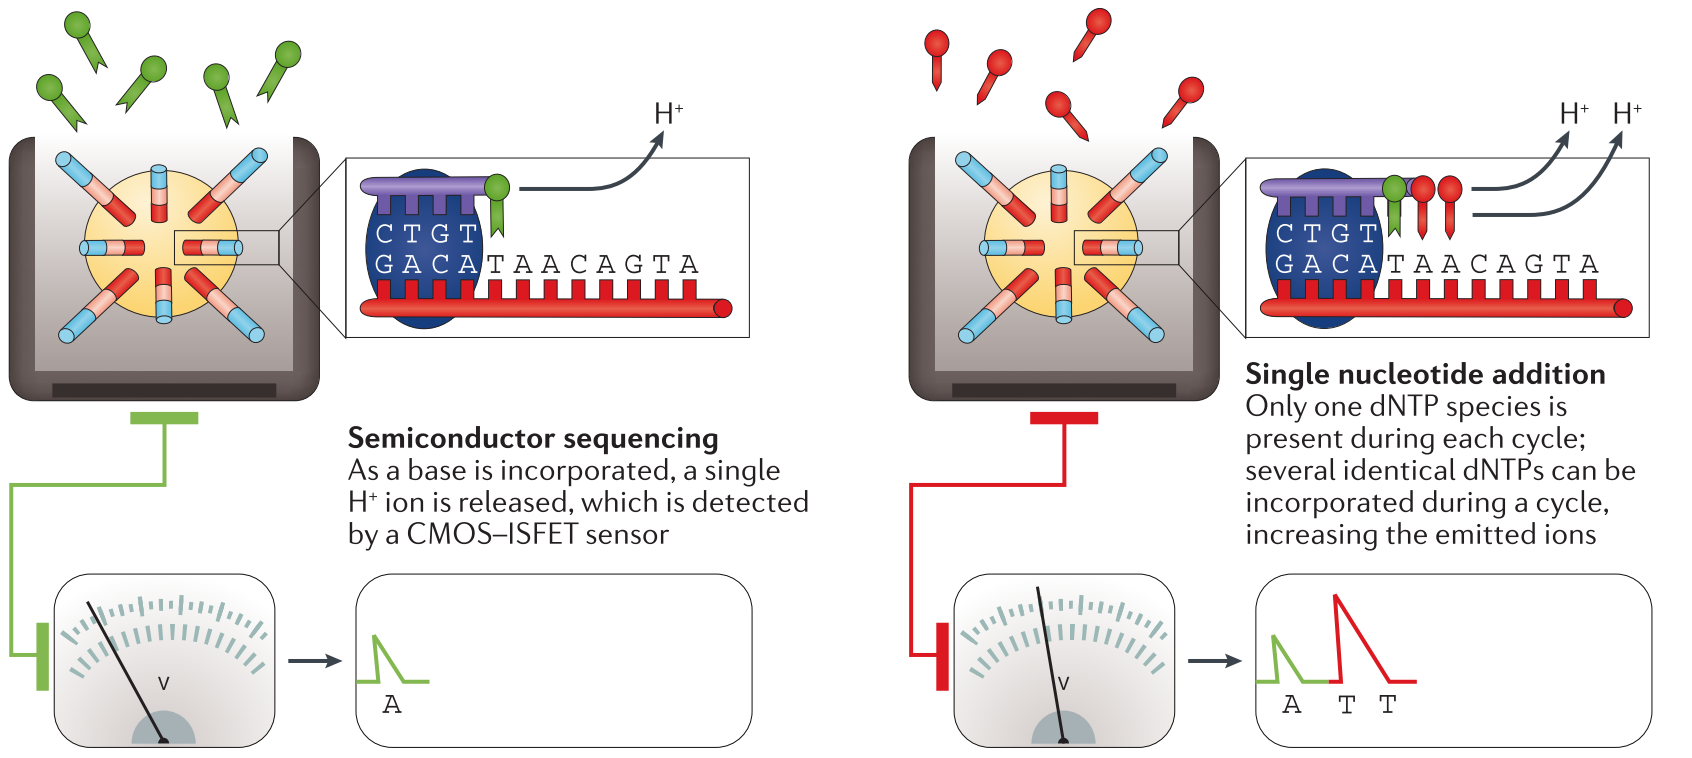
\includegraphics[scale=.26]{figure/SNA_seq_ionTorrent} 
  
  }
  
  \caption[Exemple de séquençage SNA tel qu'il est effectué par Ion Torrent]{Exemple de séquençage SNA tel qu'il est effectué par Ion Torrent d'après [@Goodwin2016] : **a** : Mise en présence du patron d'ADN à séquencer avec un mix contenant un seul type de dNTP, si le dNTP est complémentaire au patron, il se fixe et libère un proton permettant d'identifier la liaison. **b** : Dans d'homopolymère, plusieurs nucléotides identiques succesifs, autant de proton sont relaché que de constituant de bases constituant l'homopolymère, le signal émmit est donc plus fort permettant d'identifier le nombre des dNTPS liés}\label{fig:snaSeq}
  \end{figure}
  
  \begin{enumerate}
  \def\labelenumi{\arabic{enumi}.}
  \setcounter{enumi}{1}
  \tightlist
  \item
    \textbf{Séquençage par ligation} (SBL) : Par définition, cette méthode
    est basée sur l'hybridation et la ligation de l'ADN (Tomkinson,
    Vijayakumar, Pascal, \& Ellenberger, 2006) d'une sonde lée à un
    fluorophore. Ce processus utilise les caractéristique de la ligase,
    une enzyme qui a pour fonction de catalyser la liaison de deux brins
    d'ADN par des liaison phosophodiester. la sonde est constitué d'une ou
    deux bases connues, on parle alors de \emph{one-base-encoded probes}
    ou de \emph{two-bases-encoded probes} suivis d'une succession de bases
    ``dégénérées'' ou universelle, c'est à dire, des bases capables de
    s'apparier avec n'importe laquelle des quatre bases de l'ADN.
  \end{enumerate}
  
  \begin{figure}
  
  {\centering 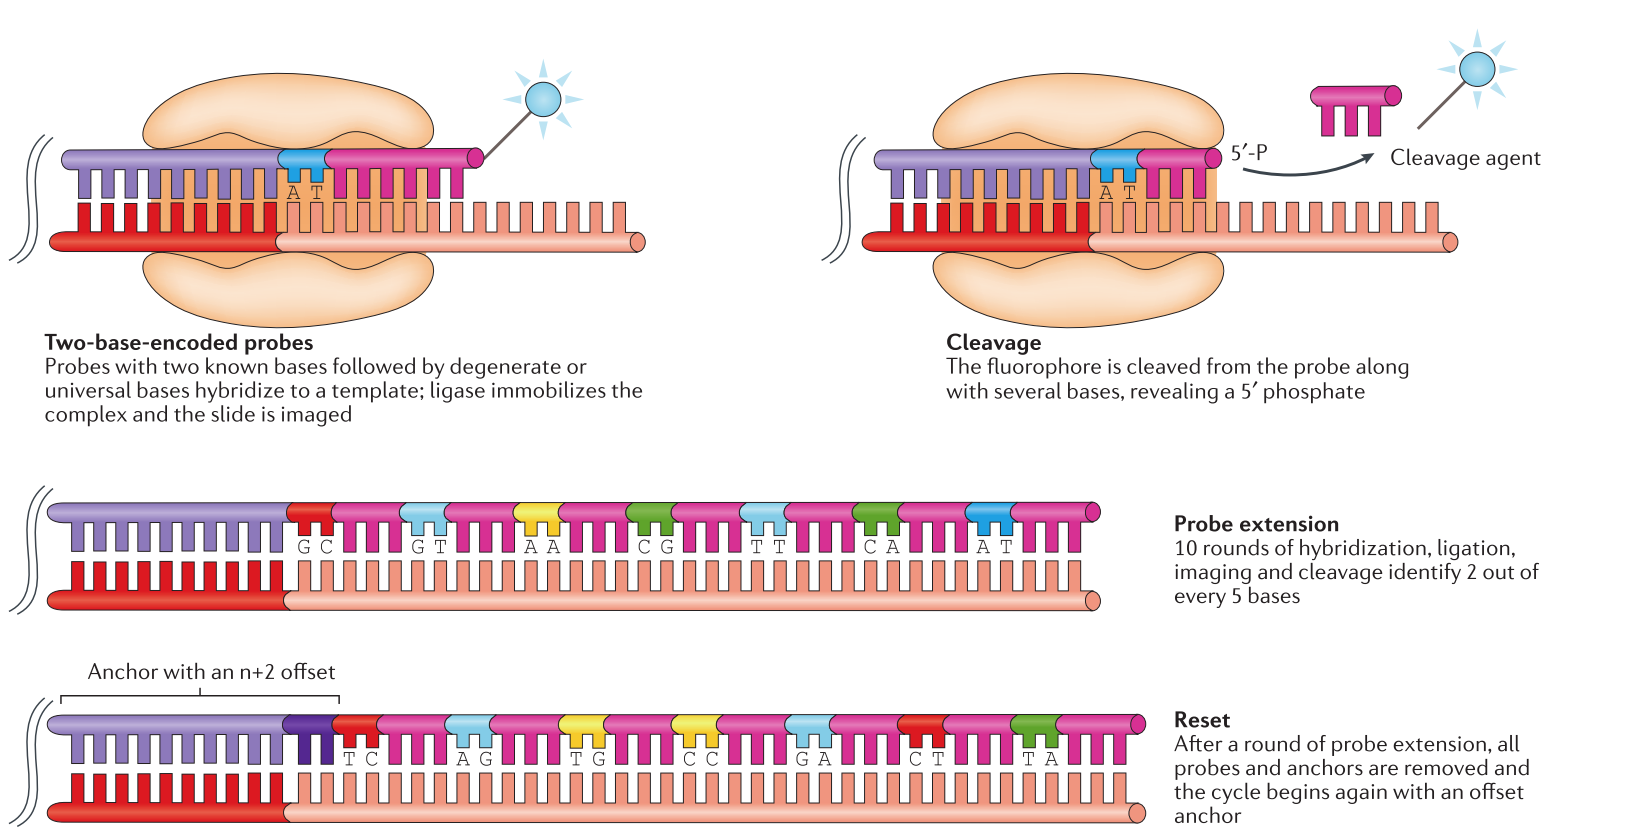
\includegraphics[scale=.26]{figure/SBL_seq_solid} 
  
  }
  
  \caption[Exemple de séquençage SBL tel qu'il est effectué par SOLiD]{Exemple de séquençage SBL tel qu'il est effectué par SOLiD d'après [@Goodwin2016] : }\label{fig:sblSeq}
  \end{figure}
  
  \section{L'analyse bioinformatique des données de
  NGS}\label{lanalyse-bioinformatique-des-donnees-de-ngs}
  
  La stratégie consistant à séquencer en parrallèle plusieurs milliers de
  \emph{reads} court a engendré plusieurs nouveaux défis bioinformatique
  dans l'analyse et l'interprétation des données de séquençage et la
  recherche de variants dans le génome humain (Wold \& Myers, 2007, M. Q.
  Yang et al. (2009)). Les\\
  Ces techniques ont été appliquées dans différents contextes, notamment
  la métagénomique (J. Qin et al., 2010), la détéction de SNPs (Van
  Tassell et al., 2008) et de variants structuraux (Alkan et al., 2010,
  Medvedev, Stanciu, \& Brudno (2009)) mais également dans des études
  portant sur la méthylation de l'ADN (K. H. Taylor et al., 2007),
  l'analyse de l'expression des ARNs messagers (Sultan et al., 2008), dans
  la génétique du cancer (Guffanti et al., 2009) et la médecine
  personalisée (Auffray, Chen, \& Hood, 2009). Cependant, pour l'ensemble
  de ces applications, la grande quantité de données générées par chaque
  analyse pose plusieurs défis informatiques (Horner et al., 2009). En
  effet, les progres techniques des dernières décénies ont rendu possible
  le séquençage de plusieurs millions des \emph{reads} d'ADN en un temps
  reliativement court et à couts raisonable. Ainsi, l'émergence du du WGS
  et du WES a permit de réunir une quantité jusqu'à présent inégalé
  d'information sur les variation génétiques, et d'une manière plus
  générale, sur les gènes et leurs fonctions ((Mardis, 2008), (Bentley,
  2006)). Cependant, de part leur nature et leur quantité, l'aquisition de
  ces nouvelles données a engendrée de nouvelles problématiques notamment
  dans l'analyse des données et leur interprétation.
  
  The number of research projects dealing with whole-genome sequencing
  data has been emerging in humans {[}3, 4, 5, 6{]}, 3 Goldstein DB, Allen
  A, Keebler J, Margulies EH, Petrou S, Petrovski S, et al. Sequencing
  studies in human genetics: design and interpretation\\
  4 Sims D, Sudbery I, Ilott NE, Heger A, Ponting CP. Sequencing depth and
  coverage: key considerations in genomic analyses. Nat Rev Genet\\
  5 Lam HYK, Clark MJ, Chen R, Chen R, Natsoulis G, O'Huallachain M, et
  al. Performance comparison of whole-genome sequencing platforms. Nat
  Biotechnol\\
  6 Morozova O, Marra M. Applications of next-generation sequencing
  technologies in functional genomics. Genomics
  
  \subsection{L'analyse des données
  brutes}\label{lanalyse-des-donnees-brutes}
  
  \hypertarget{lalignement}{\subsubsection{L'alignement}\label{lalignement}}
  
  Comme dit précédemment, le séquençage de \emph{reads} courts entraine de
  nombreuses complications et restraint l'utilisation du NGS dans de
  nombreuses applications biologiques (Wold \& Myers, 2007).
  
  L'alignement des séquences constitue probablement l'étape la plus
  importante de l'analyse des données issues du séquençage haut débit
  (Flicek \& Birney, 2009). Elle est la base sur laquelle reposent
  l'ensemble des étapes effectuées en aval, notamment l'appel des variants
  (R. Nielsen, Paul, Albrechtsen, \& Song, 2011). L'objectif de
  l'alignement est de déterminer la position correcte de chacun des
  \emph{reads} séquencés le long du génome de référence. Cette référence
  est souvent construite à partir des données de séquençage de plusieurs
  donneurs et ne représente donc pas la séquence d'un individu en
  particulier mais est sensé représenter la séquence consensus d'une
  espèce donnée. Par exemple, la séquence de référence humaine GRCh37
  (\emph{Genome Reference Consortium human build 37}) a été crées à partir
  de 13 volontaires anonymes New-Yorkais. Dès lors, cette référence
  servira de patron aux aligneurs afin qu'ils replacent correctements les
  différents \emph{reads} des l'individus séquencés.\\
  Cependant, l'étape d'alignement peut est sujette à de nombreuses erreurs
  dont certaines proviennent directement des erreurs de survenues lors de
  l'étape de séquençage, d'autres, sont dues aux caractéristiques des
  régions séquencées comme par exemple les séquence répétées (Ben Langmead
  \& Salzberg, 2012) qui pourront entrainer l'alignement d'un même
  \emph{read} à plusieurs région du génome (Treangen \& Salzberg, 2013).
  De nombreux aligneurs ont emmergé afin de répondre au mieux à cette
  problématique tel que Bowtie1(B Langmead, Trapnell, Pop, \& Salzberg,
  2009), Bowtie2 (Ben Langmead \& Salzberg, 2012), BWA, NovoAlign 2. BWA
  3. mrFAST and mrsFAST\\
  4. Novoalign\\
  5. SHRiMP\\
  6. SOAPv2
  
  \subsubsection{L'appel des variants}\label{lappel-des-variants}
  
  L'appel des variants, ou \emph{variant calling}, fait référence à
  l'ensemble des méthodes permettant d'identifier des SNVs ou des indels à
  partir des résultats de l'alignement. On appelera variants toutes
  différences de séquence observées entre un individu et la séquence de
  référence utilisée. De nombreux logiciels d'appel des variants, ou
  \emph{caller}, basés sur des algorithmes différents ont emmergés ces
  dernières années pour répondre à cette problématique. Parmis les plus
  connus on note SAMtools (H. Li et al., 2009), Genome Analysis Tool Kit -
  HaplotypeCaller (GATK-HC) (McKenna et al., 2010), Freebayes, SOAPindel
  et tvc . Les quatre premiers cités, peuvent être utilisés pour analyser
  des données provenant de tout type de plateforme de séquençage
  contrairement à TVC qui a été dévoeloppé spécifiquement pour les données
  provenant de Ion Proton. Les données issues de NGS peuvent présenter un
  taux d'erreur important. Ce taux d'erreur est multi-factorielles et
  inclus nottament les erreurs de l'alignement. L'un des éléments clef à
  prendre en compte pour pouvoir effectuer un appel de qualité est la
  couverture de la position appelée (Sims et al., 2014). Cependant, malgré
  la prise en compte de cet élément, l'appel de variants reste un
  processus dificille souvent lié à plusieurs erreurs. Plusieurs de ces
  erreurs sont même directement liées à la plateforme de séquençage
  utilisée en amont, et les différents logiciels ne présentent pas les
  même performances en fonction de ces différentes plateforme (Hwang, Kim,
  Lee, \& Marcotte, 2015), c'est pourquoi il convient d'adapter le
  logiciel d'appel en fonction de la plateforme de séquençage utilisée
  préalablement. Les erreurs d'appel sont généralement classées en deux
  catégories principales et certains aligneurs auront tendance à être plus
  sujets à l'un de ces types d'erreur qu'à l'autre (\textbf{Figure :
  }\ref{fig:snperror}) :
  
  \begin{enumerate}
  \def\labelenumi{\arabic{enumi}.}
  \tightlist
  \item
    Oubli de l'allele de référence (\textbf{IR}, \emph{ignore the
    reference allele}) : représente un variant appelé homozygote
    correspondant en réalité à un variant hétérozygote composé de l'allèle
    de référence et d'un allèle variant.\\
  \item
    Ajout de l'allèle de référence (\textbf{AR}, \emph{adding the
    reference allele}) : représente un variant appelé hétérozygote composé
    de l'allèle de référence et d'un allèle variant correspondant en
    réalité à un variant homozygote composé de deux allèles variants.\\
  \end{enumerate}
  
  \begin{figure}
  
  {\centering 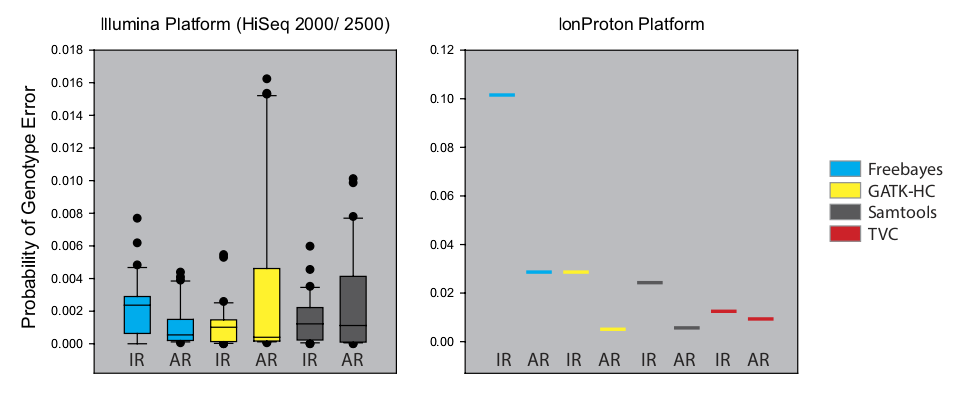
\includegraphics[scale=.50]{figure/snp_error_type} 
  
  }
  
  \caption[Représentation des erreurs d'appel de type IR et AR en fonction de la platforme de séquençage et du logiciel d'appel, d'après n Hwang et al 2015]{Représentation des erreurs d'appel de type IR et AR en fonction de la platforme de séquençage et du logiciel d'appel, d'après n Hwang et al 2015 : Pour les plateforme Illumina, on peut voir que Freebayes préfère les appels variant-homozygote tandis que GATK-HC et Samtools préfèrent les appels hétérozygotes. Pour la plateforme Ion Proton, les 4 logiciels ont une préférence pour les erreurs de type IR}\label{fig:snperror}
  \end{figure}
  
  De même que pour l'aligneur, le choix du logiciel d'appel est crutial
  car il existe de nombreuses différences dans les variants appelés par
  différents logiciels se basant sur les mêmes données brutes (Baes et
  al., 2014, O'Rawe et al. (2013), Rosenfeld, Mason, Smith, Wallin, \&
  Diekhans (2012)). En effet, en 2013, une étude comparant les réssultats
  de 5 \emph{caller} montrait que seulement 57,4\% des variants étaient
  appelés par les 5 \emph{caller} et que 80,7\% des variants étaient
  appelés par au moins 3 d'entre eux. Ce taux justait drastiquement pour
  les indels puisque la concordance était cette fois seulement de 26,8\%
  pour les indels non retrouvés par les 3 \emph{caller} (O'Rawe et al.,
  2013). Ces résultats sont cependant à pondérés avec une étude de 2015
  comparant 4 \emph{caller} et montrant que 91,7\% des SNVs séqeuencés sur
  une plateforme Illumina étaient appelés par 3 \emph{caller}, cependant,
  pour les variants séquencés sur Ion Proton, seulement 27,3\% des
  variants étaient appelés par au moins 3 \emph{caller} et 57,4\% des
  variants n'étaient appelés que par un seul des \emph{caller} (Hwang et
  al., 2015).
  
  \subsection{L'annotation des variants, filtrage et
  priorisation}\label{lannotation-des-variants-filtrage-et-priorisation}
  
  The main objective of this process is to gather substantial information
  at the variant and the gene levels. This will include the variants' data
  quality, their localization at the genomic, gene and transcripts levels,
  their genotype, their frequency in the general population, their impact
  at the mRNA and protein levels, the conservation among species of the
  affected protein residues, the variant pathogenicity prediction, and
  reported associations with diseases. At the gene level, they include the
  gene function, its spatiotemporal expression pattern, its involvement in
  various pathways, and its involvement in various phenotypes/diseases.
  
  L'annotation des variants a pour but de replacer l'ensemble des variants
  identifiés lors de l'étape d'appel dans leur contexte biologique. Elle
  vise à réunir le maximum d'information disponible à propos d'un variant
  et des unités génétiques (gènes ou transcrits) qu'il impacte. Cette
  phase est une des clefs de l'analyse puisqu'elle permet de prioriser des
  variants d'interet et de filtrer d'autres variants considérés comme non
  informatifs dans un cadre donné. Comme pour l'ensemble des étapes
  précédantes, les logiciels et jeux de données utilisés lors de l'étape
  d'annotation doivent être choisis consciencieusement, les résultats
  étant grandement impactés par ceux-ci (McCarthy et al., 2014). Cette
  annotation se fait généralement à deux niveau : 1. Au niveau du variant
  : Regroupe l'ensemble des informations concèrnant un variant donné tel
  que sa qualité, son génotype et sa fréquence 2. Au niveau de l'unité
  génétique : Regroupe les information disponible sur l'unité génétique
  impacté par le variant tel que sa fonction, son expression tissulaire,
  les voies métaboliques dans lesquelles elle est impliquée, les
  pathologies auxquelles elle est associées \emph{etc}\ldots{}
  
  \subsubsection{Au niveau du variant}\label{au-niveau-du-variant}
  
  Plusieurs informations peuvent être liées à un variant donné.
  
  \paragraph{par la fréquence : (ExAC)}\label{par-la-frequence-exac}
  
  Large consortia (e.g the human genome project {[}12, 13{]}) have been
  established to accumulate available resources, detect new variants in
  genomes, better understand genetic architecture of different traits and
  find or narrow down positions of potential causal loci
  
  12 International Human Genome Sequencing Consortium. Initial sequencing
  and analysis of the human genome\\
  13 International Human Genome Sequencing Consortium. Finishing the
  euchromatic sequence of the human genome
  
  \paragraph{Par l'impact :}\label{par-limpact}
  
  VEP SNPEFF\ldots{}
  
  SIFT,polyPhen CADD
  
  \begin{figure}
  
  {\centering 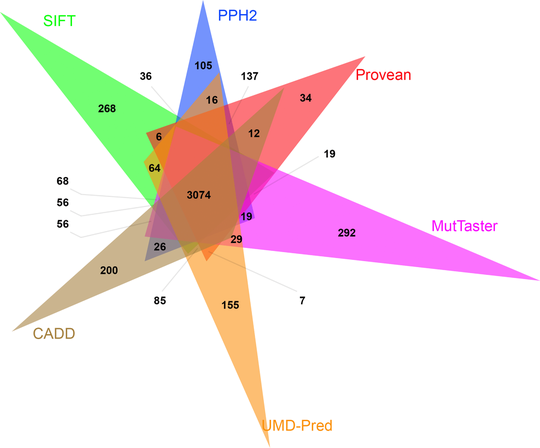
\includegraphics[scale=.7]{figure/venn_Diag_patho_pred} 
  
  }
  
  \caption[Diagramme de Venn des prédictions de pathogénicités de six logiciels d’après Salgado et al. (2016)]{Diagramme de Venn des prédictions de pathogénicités de six logiciels d’après Salgado et al. (2016) : aaaaaaaaaaaaaaaaaaaaaaaa}\label{fig:vennpred}
  \end{figure}
  
  \subsubsection{Au niveau du gène}\label{au-niveau-du-gene}
  
  L'annotation au niveau du gène (ou du transcrit) consiste à récupérer
  l'ensemble des information disponible sur le gène (impacté par le
  variant) et non plus sur le variant directement. Cette étape permet donc
  de filtrer ou de prioriser l'ensemble des variants chevauchant un gène
  (ou transcrit) donnée. L'ensemble de ces informations est donc
  extrêmement dépendante du jeux de gène utilisé et peuvent donc variaer
  en fonction de celui-ci (McCarthy et al., 2014,Zhao \& Zhang (2015))
  même si les gènes CCDS sont bien représentés à la fois par le NCBI,
  Ensembl et UCSC (Pruitt et al., 2009)
  
  Expression du gene\\
  Pathway impliquant le gene : Panther,
  
  score pour le gene : RVIS, PLI, Loftool\ldots{}
  
  HPO, OMIM
  
  RVIS, pLI
  
  Plus récemment, favorisé par l'emmergence des bases de données de
  variants, tel que ESP {[}cite{]} 1kg{[}cite{]} et surtout ExAC
  {[}cite{]}, sont apparus des scores
  
  \subsection{Conclusion NGS}\label{conclusion-ngs}
  
  En moins de 10 ans, les technologies NGS sont passées du séquençage de
  panel de gènes (environs 100 Mb pour le Roche GS FLX system) au
  séquençage de génome entiers (environs 1500 GB pour l'Illumina Hiseq
  4000) et d'une utilisation exclusive à la recherche à la routine
  clinique. Cependant, et ce malgré son succès dans le domaine de la
  génomique et de la post-génomique, plusieurs problématiques découlent de
  cette technologies. il reste au NGS plusieurs problématiques à résoudres
  
  Cependant, cette quantité de donnée produites crées de nouvelles
  problématiques pour les généticiens qui se retrouvent désormais face au
  ``déluge de données génétiques'' (Schatz \& Langmead, 2013) ce qui se
  retrouve être un frein dans la compréhension et l'interprétation des
  réseaux de gènes et leurs implication dans des pathologies, lLa
  limitation de cette technologie n'étant plus le séquençage d'un, de
  plusieurs, ou de l'ensemble des gènes, mais plutôt l'analyse et
  l'inerprétation de la masse de donnée générée.
  
  De même, nous avons pu voir que le séquençage par NGS se déroulait en
  plusieurs étapes mellant à la fois des techniqus de biologie moléculaire
  pour l'amplification par exemple, et des techniques d'informatiques et
  mathématiques, comme pour l'alignement.
  
  De nombreux efforts sont fait pour palier la contrainte instaurée par
  les \emph{reads} courts dans le cadre d'analyse génomique, cependant les
  solutions informatique et bioinformatique proposée jusqu'à présent sont
  bien en dessous des besoins créés pour l'analyse des données NGS (J. D.
  McPherson, 2009).
  
  Le séquençage nouvelle génération (NGS) a apporté avec lui des
  opportunités sans précédent dans le domaine de la recherche en
  génomique. Il a pu être appliqué à une grande variété de contexte avec
  nottament le séquençage de génome entier, ou \emph{Whole Genome
  Sequencing} (WGS) ou encore le séquençage exonique, le \emph{Whole Exome
  Sequencing} (WES). Cependant, certaines de ses caractéristiques
  techniques tel que la production de plusieurs milliards de
  \textbf{\emph{reads} courts}, bien quelles soient en partie responsable
  de son succès, sont aussi à l'origine de nouvelle problématique,
  notamment dans l'analyse et l'interprétation des données.
  
  cf Evaluation of next-generation sequencing software in mapping and
  assembly partie CHALLENGES AND PROSPECTS
  
  )
  
  \chapter{Investigation génétique et physiologique de la
  globozoospermie}\label{globo}
  
  \chapter{MutaScript}\label{mutascript}
  
  \chapter*{Conclusion}\label{conclusion}
  \addcontentsline{toc}{chapter}{Conclusion}
  
  \appendix
  
  \chapter{The First Appendix}\label{the-first-appendix}
  
  \textbf{In the main Rmd file}
  
  \textbf{In Chapter \ref{ref-labels}:}
  
  \chapter{The Second Appendix, for
  Fun}\label{the-second-appendix-for-fun}
  
  \backmatter
  
  \chapter*{References}\label{references}
  \addcontentsline{toc}{chapter}{References}
  
  \noindent
  
  \setlength{\parindent}{-0.20in} \setlength{\leftskip}{0.20in}
  \setlength{\parskip}{8pt}
  
  \hypertarget{refs}{}
  \hypertarget{ref-Adelman1989}{}
  Adelman, M. M., \& Cahill, E. M. (1989). \emph{Atlas of sperm
  morphology} (p. 123). ASCP Press.
  
  \hypertarget{ref-Alkan2010}{}
  Alkan, C., Kidd, J. M., Marques-bonet, T., Aksay, G., Hormozdiari, F.,
  Kitzman, J. O., \ldots{} Eichler, E. E. (2010). Personalized Copy-Number
  and Segmental Duplication Maps using Next-Generation Sequencing.
  \emph{Nature Genetics}, \emph{41}(10), 1061--1067.
  \url{http://doi.org/10.1038/ng.437.Personalized}
  
  \hypertarget{ref-Asimakopoulos2003}{}
  Asimakopoulos, B. (2003). Is There a Place for Round and Elongated
  Spermatids Injection in, \emph{1}(1), 1--6.
  
  \hypertarget{ref-Auffray2009}{}
  Auffray, C., Chen, Z., \& Hood, L. (2009). Systems medicine: the future
  of medical genomics and healthcare. \emph{Genome Medicine}, \emph{1}(1),
  2. \url{http://doi.org/10.1186/gm2}
  
  \hypertarget{ref-Baes2014}{}
  Baes, C. F., Dolezal, M. A., Koltes, J. E., Bapst, B., Fritz-Waters, E.,
  Jansen, S., \ldots{} Gredler, B. (2014). Evaluation of variant
  identification methods for whole genome sequencing data in dairy cattle.
  \emph{BMC Genomics}, \emph{15}(1), 948.
  \url{http://doi.org/10.1186/1471-2164-15-948}
  
  \hypertarget{ref-Bentley2006}{}
  Bentley, D. R. (2006). Whole-genome re-sequencing. \emph{Current Opinion
  in Genetics and Development}, \emph{16}(6), 545--552.
  \url{http://doi.org/10.1016/j.gde.2006.10.009}
  
  \hypertarget{ref-Cho2001}{}
  Cho, C., Willis, W. D., Goulding, E. H., Jung-Ha, H., Choi, Y. C.,
  Hecht, N. B., \& Eddy, E. M. (2001). Haploinsufficiency of protamine-1
  or -2 causes infertility in mice. \emph{Nature Genetics}, \emph{28}(1),
  82--6. \url{http://doi.org/10.1038/88313}
  
  \hypertarget{ref-Clermont1963}{}
  Clermont, Y. (1963). The cycle of the seminiferous epithelium in man.
  \emph{American Journal of Anatomy}, \emph{112}(1), 35--51.
  \url{http://doi.org/10.1002/aja.1001120103}
  
  \hypertarget{ref-Clermont1966}{}
  Clermont, Y. (1966). Renewal of spermatogonia in man. \emph{American
  Journal of Anatomy}, \emph{118}(2), 509--524.
  \url{http://doi.org/10.1002/aja.1001180211}
  
  \hypertarget{ref-Collins2003}{}
  Collins, F. S., Morgan, M., \& Patrinos, A. (2003). The Human Genome
  Project: Lessons from Large-Scale Biology. \emph{Science},
  \emph{300}(5617), 286--290. \url{http://doi.org/10.1126/science.1084564}
  
  \hypertarget{ref-Eddy2007}{}
  Eddy, E. M. (2007). The scaffold role of the fibrous sheath.
  \emph{Society of Reproduction and Fertility Supplement}, \emph{65},
  45--62. Retrieved from \url{http://www.ncbi.nlm.nih.gov/pubmed/17644954}
  
  \hypertarget{ref-Escalier1991}{}
  Escalier, D., Gallo, J. M., Albert, M., Meduri, G., Bermudez, D., David,
  G., \& Schrevel, J. (1991). Human acrosome biogenesis: immunodetection
  of proacrosin in primary spermatocytes and of its partitioning pattern
  during meiosis. \emph{Development (Cambridge, England)}, \emph{113}(3),
  779--788. Retrieved from
  \url{http://dev.biologists.org/content/develop/113/3/779.full.pdf}
  
  \hypertarget{ref-Flicek2009}{}
  Flicek, P., \& Birney, E. (2009). Sense from sequence reads: methods for
  alignment and assembly. \emph{Nature Methods}, \emph{6}(11 Suppl),
  S6--S12. \url{http://doi.org/10.1038/nmeth0610-479b}
  
  \hypertarget{ref-Gnessi1997}{}
  Gnessi, L., Fabbri, A., \& Spera, G. (1997). Gonadal peptides as
  mediators of development and functional control of the testis: An
  integrated system with hormones and local environment. \emph{Endocrine
  Reviews}, \emph{18}(4), 541--609.
  \url{http://doi.org/10.1210/er.18.4.541}
  
  \hypertarget{ref-Goodwin2016}{}
  Goodwin, S., McPherson, J. D., \& McCombie, W. R. (2016). Coming of age:
  ten years of next-generation sequencing technologies. \emph{Nat Rev
  Genet}, \emph{17}(6), 333--351. \url{http://doi.org/10.1038/nrg.2016.49}
  
  \hypertarget{ref-Goossens2013}{}
  Goossens, E., \& Tournaye, H. (2013). Adult stem cells in the human
  testis. \emph{Seminars in Reproductive Medicine}, \emph{31}(1), 39--48.
  \url{http://doi.org/10.1055/s-0032-1331796}
  
  \hypertarget{ref-Guffanti2009}{}
  Guffanti, A., Iacono, M., Pelucchi, P., Kim, N., Soldà, G., Croft, L.
  J., \ldots{} De Bellis, G. (2009). A transcriptional sketch of a primary
  human breast cancer by 454 deep sequencing. \emph{BMC Genomics},
  \emph{10}(1), 163. \url{http://doi.org/10.1186/1471-2164-10-163}
  
  \hypertarget{ref-Guo2008}{}
  Guo, J., Xu, N., Li, Z., Zhang, S., Wu, J., Kim, D. H., \ldots{} Ju, J.
  (2008). Four-color DNA sequencing with 3'-O-modified nucleotide
  reversible terminators and chemically cleavable fluorescent
  dideoxynucleotides. \emph{Proceedings of the National Academy of
  Sciences of the United States of America}, \emph{105}(27), 9145--9150.
  \url{http://doi.org/10.1073/pnas.0804023105}
  
  \hypertarget{ref-Hamilton1987}{}
  Hamilton, D. W., Waites, G. M. H. (1990). \emph{Cellular and Molecular
  Events in Spermiogenesis} (p. 334). Cambridge University Press.
  Retrieved from
  \url{http://www.cambridge.org/us/academic/subjects/medicine/obstetrics-and-gynecology-reproductive-medicine/cellular-and-molecular-events-spermiogenesis}
  
  \hypertarget{ref-Hermo2010}{}
  Hermo, L., Pelletier, R. M., Cyr, D. G., \& Smith, C. E. (2010). Surfing
  the wave, cycle, life history, and genes/proteins expressed by
  testicular germ cells. Part 3: Developmental changes in spermatid
  flagellum and cytoplasmic droplet and interaction of sperm with the zona
  pellucida and egg plasma membrane. \emph{Microscopy Research and
  Technique}, \emph{73}(4), 320--363.
  \url{http://doi.org/10.1002/jemt.20784}
  
  \hypertarget{ref-Horner2009}{}
  Horner, D. S., Pavesi, G., Castrignano', T., Meo, P. D. O. de, Liuni,
  S., Sammeth, M., \ldots{} Pesole, G. (2009). Bioinformatics approaches
  for genomics and post genomics applications of next-generation
  sequencing. \emph{Briefings in Bioinformatics}, \emph{11}(2), 181--197.
  \url{http://doi.org/10.1093/bib/bbp046}
  
  \hypertarget{ref-Hwang2015}{}
  Hwang, S., Kim, E., Lee, I., \& Marcotte, E. M. (2015). Systematic
  comparison of variant calling pipelines using gold standard personal
  exome variants. \emph{Scientific Reports}, \emph{5}(December), 17875.
  \url{http://doi.org/10.1038/srep17875}
  
  \hypertarget{ref-Inaba2003}{}
  Inaba, K. (2003). Molecular Architecture of the Sperm Flagella:
  Molecules for Motility and Signaling. \emph{Zoological Science},
  \emph{20}(9), 1043--1056. \url{http://doi.org/10.2108/zsj.20.1043}
  
  \hypertarget{ref-Johnson1980}{}
  JOHNSON, L., PETTY, C. S., \& NEAVES, W. B. (1980). A Comparative Study
  of Daily Sperm Production and Testicular Composition in Humans and Rats.
  \emph{Biol Reprod}, \emph{22}(5), 1233--1243. Retrieved from
  \url{http://www.biolreprod.org/content/22/5/1233.short}
  
  \hypertarget{ref-KIERSZENBAUM1994}{}
  KIERSZENBAUM, A. L. (1994). Mammalian Spermatogenesis
  \textless{}i\textgreater{}in Vivo\textless{}/i\textgreater{} and
  \textless{}i\textgreater{}in Vitro\textless{}/i\textgreater{} : A
  Partnership of Spermatogenic and Somatic Cell Lineages*. \emph{Endocrine
  Reviews}, \emph{15}(1), 116--134.
  \url{http://doi.org/10.1210/edrv-15-1-116}
  
  \hypertarget{ref-Kierszenbaum1978}{}
  Kierszenbaum, A. L., \& Tres, L. L. (1978). RNA transcription and
  chromatin structure during meiotic and postmeiotic stages of
  spermatogenesis. \emph{Federation Proceedings}, \emph{37}(11), 2512--6.
  Retrieved from \url{http://www.ncbi.nlm.nih.gov/pubmed/357185}
  
  \hypertarget{ref-Langmead2012}{}
  Langmead, B., \& Salzberg, S. L. (2012). Fast gapped-read alignment with
  Bowtie 2. \emph{Nature Methods}, \emph{9}(4), 357--359.
  \url{http://doi.org/10.1038/nmeth.1923}
  
  \hypertarget{ref-Langmead2009}{}
  Langmead, B., Trapnell, C., Pop, M., \& Salzberg, S. (2009). Ultrafast
  and memory-efficient alignment of short DNA sequences to the human
  genome. \emph{Genome Biology}, \emph{10}(3), R25.
  \url{http://doi.org/10.1186/gb-2009-10-3-r25}
  
  \hypertarget{ref-Lelieveld2015}{}
  Lelieveld, S. H., Spielmann, M., Mundlos, S., Veltman, J. a, \&
  Gilissen, C. (2015). Comparison of Exome and Genome Sequencing
  Technologies for the Complete Capture of Protein-Coding Regions.
  \emph{Human Mutation}, \emph{36}(8), 815--22.
  \url{http://doi.org/10.1002/humu.22813}
  
  \hypertarget{ref-Li2009}{}
  Li, H., Handsaker, B., Wysoker, A., Fennell, T., Ruan, J., Homer, N.,
  \ldots{} Durbin, R. (2009). The Sequence Alignment/Map format and
  SAMtools. \emph{Bioinformatics}, \emph{25}(16), 2078--2079.
  \url{http://doi.org/10.1093/bioinformatics/btp352}
  
  \hypertarget{ref-Mardis2008}{}
  Mardis, E. R. (2008). The impact of next-generation sequencing
  technology on genetics. \emph{Trends in Genetics}, \emph{24}(3),
  133--141. \url{http://doi.org/10.1016/j.tig.2007.12.007}
  
  \hypertarget{ref-McCarthy2014}{}
  McCarthy, D. J., Humburg, P., Kanapin, A., Rivas, M. a, Gaulton, K.,
  Cazier, J.-B., \& Donnelly, P. (2014). Choice of transcripts and
  software has a large effect on variant annotation. \emph{Genome
  Medicine}, \emph{6}(3), 26. \url{http://doi.org/10.1186/gm543}
  
  \hypertarget{ref-McKenna2010}{}
  McKenna, A., Hanna, M., Banks, E., Sivachenko, A., Cibulskis, K.,
  Kernytsky, A., \ldots{} DePristo, M. A. (2010). The Genome Analysis
  Toolkit: a MapReduce framework for analyzing next-generation DNA
  sequencing data. \emph{Genome Research}, \emph{20}(9), 1297--303.
  \url{http://doi.org/10.1101/gr.107524.110}
  
  \hypertarget{ref-McPherson2009}{}
  McPherson, J. D. (2009). Next-generation gap. \emph{Nature Methods},
  \emph{6}(11s), S2--S5. \url{http://doi.org/10.1038/nmeth.f.268}
  
  \hypertarget{ref-Medvedev2009}{}
  Medvedev, P., Stanciu, M., \& Brudno, M. (2009). Computational methods
  for discovering structural variation with next-generation sequencing.
  \emph{Nature Methods}, \emph{6}(11s), S13--S20.
  \url{http://doi.org/10.1038/nmeth.1374}
  
  \hypertarget{ref-Meienberg2016}{}
  Meienberg, J., Bruggmann, R., Oexle, K., \& Matyas, G. (2016). Clinical
  sequencing: is WGS the better WES? \emph{Human Genetics}, \emph{135}(3),
  359--362. \url{http://doi.org/10.1007/s00439-015-1631-9}
  
  \hypertarget{ref-Metzker2010}{}
  Metzker, M. L. (2010). Sequencing technologies - the next generation.
  \emph{Nature Reviews. Genetics}, \emph{11}(1), 31--46.
  \url{http://doi.org/10.1038/nrg2626}
  
  \hypertarget{ref-Ng2010}{}
  Ng, S. B., Turner, E. H., Robertson, P. D., Flygare, S. D., Abigail, W.,
  Lee, C., \ldots{} Shendure, J. (2010). Targeted Capture and Massicely
  Parallel Sequencing of twelve human exomes. \emph{Nature},
  \emph{461}(7261), 272--276.
  \url{http://doi.org/10.1038/nature08250.Targeted}
  
  \hypertarget{ref-Nielsen2011}{}
  Nielsen, R., Paul, J. S., Albrechtsen, A., \& Song, Y. S. (2011).
  Genotype and SNP calling from next-generation sequencing data.
  \emph{Nature Reviews. Genetics}, \emph{12}(6), 443--51.
  \url{http://doi.org/10.1038/nrg2986}
  
  \hypertarget{ref-Ogura1994}{}
  Ogura, a, Matsuda, J., \& Yanagimachi, R. (1994). Birth of normal young
  after electrofusion of mouse oocytes with round spermatids.
  \emph{Proceedings of the National Academy of Sciences of the United
  States of America}, \emph{91}(16), 7460--7462.
  \url{http://doi.org/10.1073/pnas.91.16.7460}
  
  \hypertarget{ref-Kimura1995}{}
  Ogura, A., Matsuda, J., Asano, T., Suzuki, O., \& Yanagimachi, R.
  (1996). Mouse oocytes injected with cryopreserved round spermatids can
  develop into normal offspring. \emph{Journal of Assisted Reproduction
  and Genetics}, \emph{13}(5), 431--434.
  \url{http://doi.org/10.1007/BF02066177}
  
  \hypertarget{ref-ORawe2013}{}
  O'Rawe, J., Jiang, T., Sun, G., Wu, Y., Wang, W., Hu, J., \ldots{} Lyon,
  G. J. (2013). Low concordance of multiple variant-calling pipelines:
  practical implications for exome and genome sequencing. \emph{Genome
  Medicine}, \emph{5}(3), 28. \url{http://doi.org/10.1186/gm432}
  
  \hypertarget{ref-Papic}{}
  Papic, Z., Katona, G., \& Skrabalo, Z. (1988). The cytologic
  identification and quantification of testicular cell subtypes.
  Reproducibility and relation to histologic findings in the diagnosis of
  male infertility. \emph{Acta Cytologica}, \emph{32}(5), 697--706.
  Retrieved from \url{http://www.ncbi.nlm.nih.gov/pubmed/3421018}
  
  \hypertarget{ref-Pedersen1974}{}
  Pedersen, H., \& Rebbe, H. (1974). Fine structure of round-headed human
  spermatozoa. \emph{Journal of Reproduction and Fertility}, \emph{37}(1),
  51--4. \url{http://doi.org/10.1530/JRF.0.0370051}
  
  \hypertarget{ref-Pruitt2009}{}
  Pruitt, K. D., Harrow, J., Harte, R. A., Wallin, C., Diekhans, M.,
  Maglott, D. R., \ldots{} Lipman, D. (2009). The consensus coding
  sequence (CCDS) project: Identifying a common protein-coding gene set
  for the human and mouse genomes. \emph{Genome Research}, \emph{19}(7),
  1316--1323. \url{http://doi.org/10.1101/gr.080531.108}
  
  \hypertarget{ref-Qin2010}{}
  Qin, J., Li, R., Raes, J., Arumugam, M., Burgdorf, S., Manichanh, C.,
  \ldots{} Yang, H. (2010). A human gut microbial gene catalog established
  by metagenomic sequencing. \emph{Nature}, \emph{464}(7285), 59--65.
  \url{http://doi.org/10.1038/nature08821.A}
  
  \hypertarget{ref-Rosenfeld2012}{}
  Rosenfeld, J. A., Mason, C. E., Smith, T. M., Wallin, C., \& Diekhans,
  M. (2012). Limitations of the Human Reference Genome for Personalized
  Genomics. \emph{PLoS ONE}, \emph{7}(7), e40294.
  \url{http://doi.org/10.1371/journal.pone.0040294}
  
  \hypertarget{ref-Sasagawa}{}
  Sasagawa, I., \& Yanagimachi, R. (1997). Spermatids from mice after
  cryptorchid and reversal operations can initiate normal embryo
  development. \emph{Journal of Andrology}, \emph{18}(2), 203--209.
  Retrieved from \url{http://www.ncbi.nlm.nih.gov/pubmed/9154515}
  
  \hypertarget{ref-Schatz2013}{}
  Schatz, M. C., \& Langmead, B. (2013). The DNA Data Deluge: Fast,
  efficient genome sequencing machines are spewing out more data than
  geneticists can analyze. \emph{IEEE Spectrum}, \emph{50}(7), 26--33.
  \url{http://doi.org/10.1109/MSPEC.2013.6545119}
  
  \hypertarget{ref-Schenck}{}
  Schenck, U., \& Schill, W. B. (n.d.). Cytology of the human seminiferous
  epithelium. \emph{Acta Cytologica}, \emph{32}(5), 689--96. Retrieved
  from \url{http://www.ncbi.nlm.nih.gov/pubmed/3421017}
  
  \hypertarget{ref-Sims2014}{}
  Sims, D., Sudbery, I., Ilott, N. E., Heger, A., \& Ponting, C. P.
  (2014). Sequencing depth and coverage: key considerations in genomic
  analyses. \emph{Nature Reviews. Genetics}, \emph{15}(2), 121--32.
  \url{http://doi.org/10.1038/nrg3642}
  
  \hypertarget{ref-Singh}{}
  Singh, G. (n.d.). Ultrastructural features of round-headed human
  spermatozoa. \emph{International Journal of Fertility}, \emph{37}(2),
  99--102. Retrieved from \url{http://www.ncbi.nlm.nih.gov/pubmed/1349598}
  
  \hypertarget{ref-Sultan2008}{}
  Sultan, M., Schulz, M. H., Richard, H., Magen, A., Klingenhoff, A.,
  Scherf, M., \ldots{} Yaspo, M.-L. (2008). A Global View of Gene Activity
  and Alternative Splicing by Deep Sequencing of the Human Transcriptome.
  \emph{Science}, \emph{321}(5891), 956--960.
  \url{http://doi.org/10.1126/science.1160342}
  
  \hypertarget{ref-Tanaka2015}{}
  Tanaka, A., Nagayoshi, M., Takemoto, Y., Tanaka, I., Kusunoki, H.,
  Watanabe, S., \ldots{} Yanagimachi, R. (2015). Fourteen babies born
  after round spermatid injection into human oocytes. \emph{Proceedings of
  the National Academy of Sciences}, \emph{112}(March 2014), 201517466.
  \url{http://doi.org/10.1073/pnas.1517466112}
  
  \hypertarget{ref-Taylor2007}{}
  Taylor, K. H., Kramer, R. S., Davis, J. W., Guo, J., Duff, D. J., Xu,
  D., \ldots{} Shi, H. (2007). Ultradeep Bisulfite Sequencing Analysis of
  DNA Methylation Patterns in Multiple Gene Promoters by 454 Sequencing.
  \emph{Cancer Research}, \emph{67}(18), 8511--8518.
  \url{http://doi.org/10.1158/0008-5472.CAN-07-1016}
  
  \hypertarget{ref-Tomkinson2006}{}
  Tomkinson, A. E., Vijayakumar, S., Pascal, J. M., \& Ellenberger, T.
  (2006). DNA Ligases:~ Structure, Reaction Mechanism, and Function.
  \emph{Chemical Reviews}, \emph{106}(2), 687--699.
  \url{http://doi.org/10.1021/cr040498d}
  
  \hypertarget{ref-Treangen2013}{}
  Treangen, T. J., \& Salzberg, S. L. (2013). Repetitive DNA and
  next-generation sequencing: computational challenges and solutions.
  \emph{Nat Rev Genet.}, \emph{13}(1), 36--46.
  \url{http://doi.org/10.1038/nrg3117.Repetitive}
  
  \hypertarget{ref-VanTassell2008}{}
  Van Tassell, C. P., Smith, T. P. L., Matukumalli, L. K., Taylor, J. F.,
  Schnabel, R. D., Lawley, C. T., \ldots{} Sonstegard, T. S. (2008). SNP
  discovery and allele frequency estimation by deep sequencing of reduced
  representation libraries. \emph{Nature Methods}, \emph{5}(3), 247--252.
  \url{http://doi.org/10.1038/nmeth.1185}
  
  \hypertarget{ref-Ward1994}{}
  Ward, W. S. (1994). The structure of the sleeping genome: implications
  of sperm DNA organization for somatic cells. \emph{Journal of Cellular
  Biochemistry}, \emph{55}(1), 77--82.
  \url{http://doi.org/10.1002/jcb.240550109}
  
  \hypertarget{ref-Wold2007}{}
  Wold, B., \& Myers, R. M. (2007). Sequence census methods for functional
  genomics. \emph{Nature Methods}, \emph{5}(1), 19--21.
  \url{http://doi.org/10.1038/nmeth1157}
  
  \hypertarget{ref-WorldHealthOrganization1992}{}
  World Health Organization. (1992). \emph{WHO laboratory manual for the
  examination of human semen and sperm-cervical mucus interaction.} (3th
  ed, p. 128). Cambridge University Press.
  
  \hypertarget{ref-Yang2009}{}
  Yang, M. Q., Athey, B. D., Arabnia, H. R., Sung, A. H., Liu, Q., Yang,
  J. Y., \ldots{} Deng, Y. (2009). High-throughput next-generation
  sequencing technologies foster new cutting-edge computing techniques in
  bioinformatics. \emph{BMC Genomics}, \emph{10 Suppl 1}, I1.
  \url{http://doi.org/10.1186/1471-2164-10-S1-I1}
  
  \hypertarget{ref-Zhao2015}{}
  Zhao, S., \& Zhang, B. (2015). A comprehensive evaluation of ensembl,
  RefSeq, and UCSC annotations in the context of RNA-seq read mapping and
  gene quantification. \emph{BMC Genomics}, \emph{16}(1), 97.
  \url{http://doi.org/10.1186/s12864-015-1308-8}


  % Index?

\end{document}

